\chapter{Experimentos y evaluación}
\label{cap:experimentos}

\section{Implementación del sistema}
Para la implementación del sistema propuesto, se ha utilizado como base el sistema de procesamiento de \textit{stream} S4 \citep{s4}, cuyo modelo fue explicado en la Sección \ref{sec:SPS}. El desarrollo del modelo elástico de replicación de operadores de un SPS se ha implementando en Java, modificándose el código fuente de S4 para incluir las funcionalidades de la solución propuesta, de tal manera que sea automático y transparente para el usuario del SPS.

El sistema diseñado se ha añadido al proyecto S4, generando un paquete denominado \textit{modelo} que contiene las clases: \textit{S4Monitor}, \textit{MarkovChain}, \textit{modeloMetrics}, \textit{StatusPE} y \textit{\mbox{TopologyApp}}, para mayor información véase el Anexo \ref{apendice:clases}.

Para la ejecución del SPS en conjunto con el modelo, se debe en primer lugar registrar los PEs. Además de esto, se ha añadido a cada PE como atributo la cantidad de eventos y salientes, y también un boolean en caso que se desee sólo una réplica del operador.

%Además de lo anterior, para el análisis de cada uno de los PEs, se ha añadido los atributos correspondientes a la cantidad de eventos entrantes y salientes en un período de un segundo. Esto es utilizado posteriormente para las estadísticas utilizadas por el algoritmo reactivo y predictivo. Además, se ha agregado un atributo booleano, el cual indica si el PE puede aumentar o disminuir la cantidad de réplicas que posee. Este atributo es necesario para aquellos operadores que al replicar se hace necesario un operador auxiliar, de tal manera que éste junte las respuestas que entrega cada réplica, por lo que con este atributo el operador es único, sin poder replicarse.

%Para el funcionamiento del modelo se ejecutan dos tareas en la aplicación de S4: una tarea que guarda las muestras para el historial del operador y otra que envía las estadísticas del operador, las cuales poseen un intervalo de ejecución de 1 y 5 segundos respectivamente. La primera tarea analiza cada uno de los PEs, tomando en consideración las estadísticas de eventos entrantes y salientes, de tal manera de obtener la tasa de llegada ($\lambda$) y procesamiento ($\mu$), para posteriormente calcular la tasa de rendimiento en la ventana de tiempo analizada, guardando así la muestra en el historial. La segunda tarea obtiene las estadísticas de cada uno de los PEs, la tasa de llegada y procesamiento, dado los eventos entrantes y salientes, cantidad de eventos totales e historial del PE, los cuales son enviados al modelo de carga, para ejecutar el algoritmo que corresponda según la ventana de tiempo. Finalmente el módulo de administración de réplicas aumenta o disminuye las réplicas necesarias en cada operador. El código de la implementación se puede observar en el Anexo \ref{apendice:codigoFuenteS4}.
%
%En el caso del envío de las estadísticas, después de ser enviadas, se consulta el estado de cada uno de los operadores, y en caso de ser necesario, se realiza las modificaciones en el sistema, ya sea para crear o eliminar réplicas de un operador. Por lo que se consulta la cantidad de réplicas que estima el modelo elástico que deben existir, y en caso de ser un número de réplicas mayor que el actual, se crea la cantidad de réplicas faltantes. Por otra parte, si el número de réplicas estimado es menor, se eliminan las réplicas sobrantes, por lo que se finaliza la ejecución de las réplicas sobrantes y posteriormente las remueve. Los códigos asociados a los de creación o eliminación de réplicas se presentan en el Anexo \ref{apendice:codigoFuenteS4}.

Para el funcionamiento del modelo se ejecutan dos tareas en la aplicación de S4: una tarea que recolecta los datos y otra que recupera los resultados obtenidos por el modelo elástico. En caso que el administrador de réplicas indique se requiere modificar la cantidad de réplica, la segunda tarea realiza los cambios correspondientes al PE expresado. Los códigos asociados a los de creación o eliminación de réplicas se presentan en el Anexo \ref{apendice:codigoFuenteS4}.

Dado que en el diseño se propuso un mecanismo de balance de carga basado en la técnica de replicación, se hace necesario modificar S4, de manera de poder manejar las réplicas de los operadores. Para la distribución de eventos cuando existe más de una réplica, se aplica una política basada en el largo de la cola de los operadores, donde aquel que posea menor largo es el candidato para recibir el evento entrante. \normalsize{El componente que escoge esto, es el \textit{pipeline} que existe entre los dos operadores, el cual analiza a qué operador debe enviar el dato, según la política explicada anteriormente. Este pipeline es una clase llamada \textit{Stream}, el cual va a actuar como intermediario entre el operador emisor y receptor, de tal manera que en caso que se envíe el evento, va a pasar por esta clase y encola el evento para ser procesado posteriormente en alguna de réplicas disponibles.}

En la Figura \ref{fig:distCarga} se explica gráficamente la distribución de la carga. En la Figura \ref{fig:distCarga} (a) el operador A envía un evento al operador B, el cual posee tres réplicas, siendo \normalsize{las colas de menor tamaño} las que están en la réplica 2 y 3. Dado que el tamaño de las colas son iguales, se escoge la primera réplica disponible, es decir, la réplica 2. Posteriormente, como la réplica 2 aumenta su cola, la réplica 3 es la que posee menor cantidad de eventos en cola, como se demuestra en la Figura \ref{fig:distCarga} (b), por lo tanto, ésta es la réplica candidata a recibir el evento enviado. Finalmente, en la Figura \ref{fig:distCarga} (c) todas las réplicas poseen el mismo tamaño de la cola, por lo tanto, se procede a enviar a la primera réplica.

\begin{figure}[!ht]
	\centering
		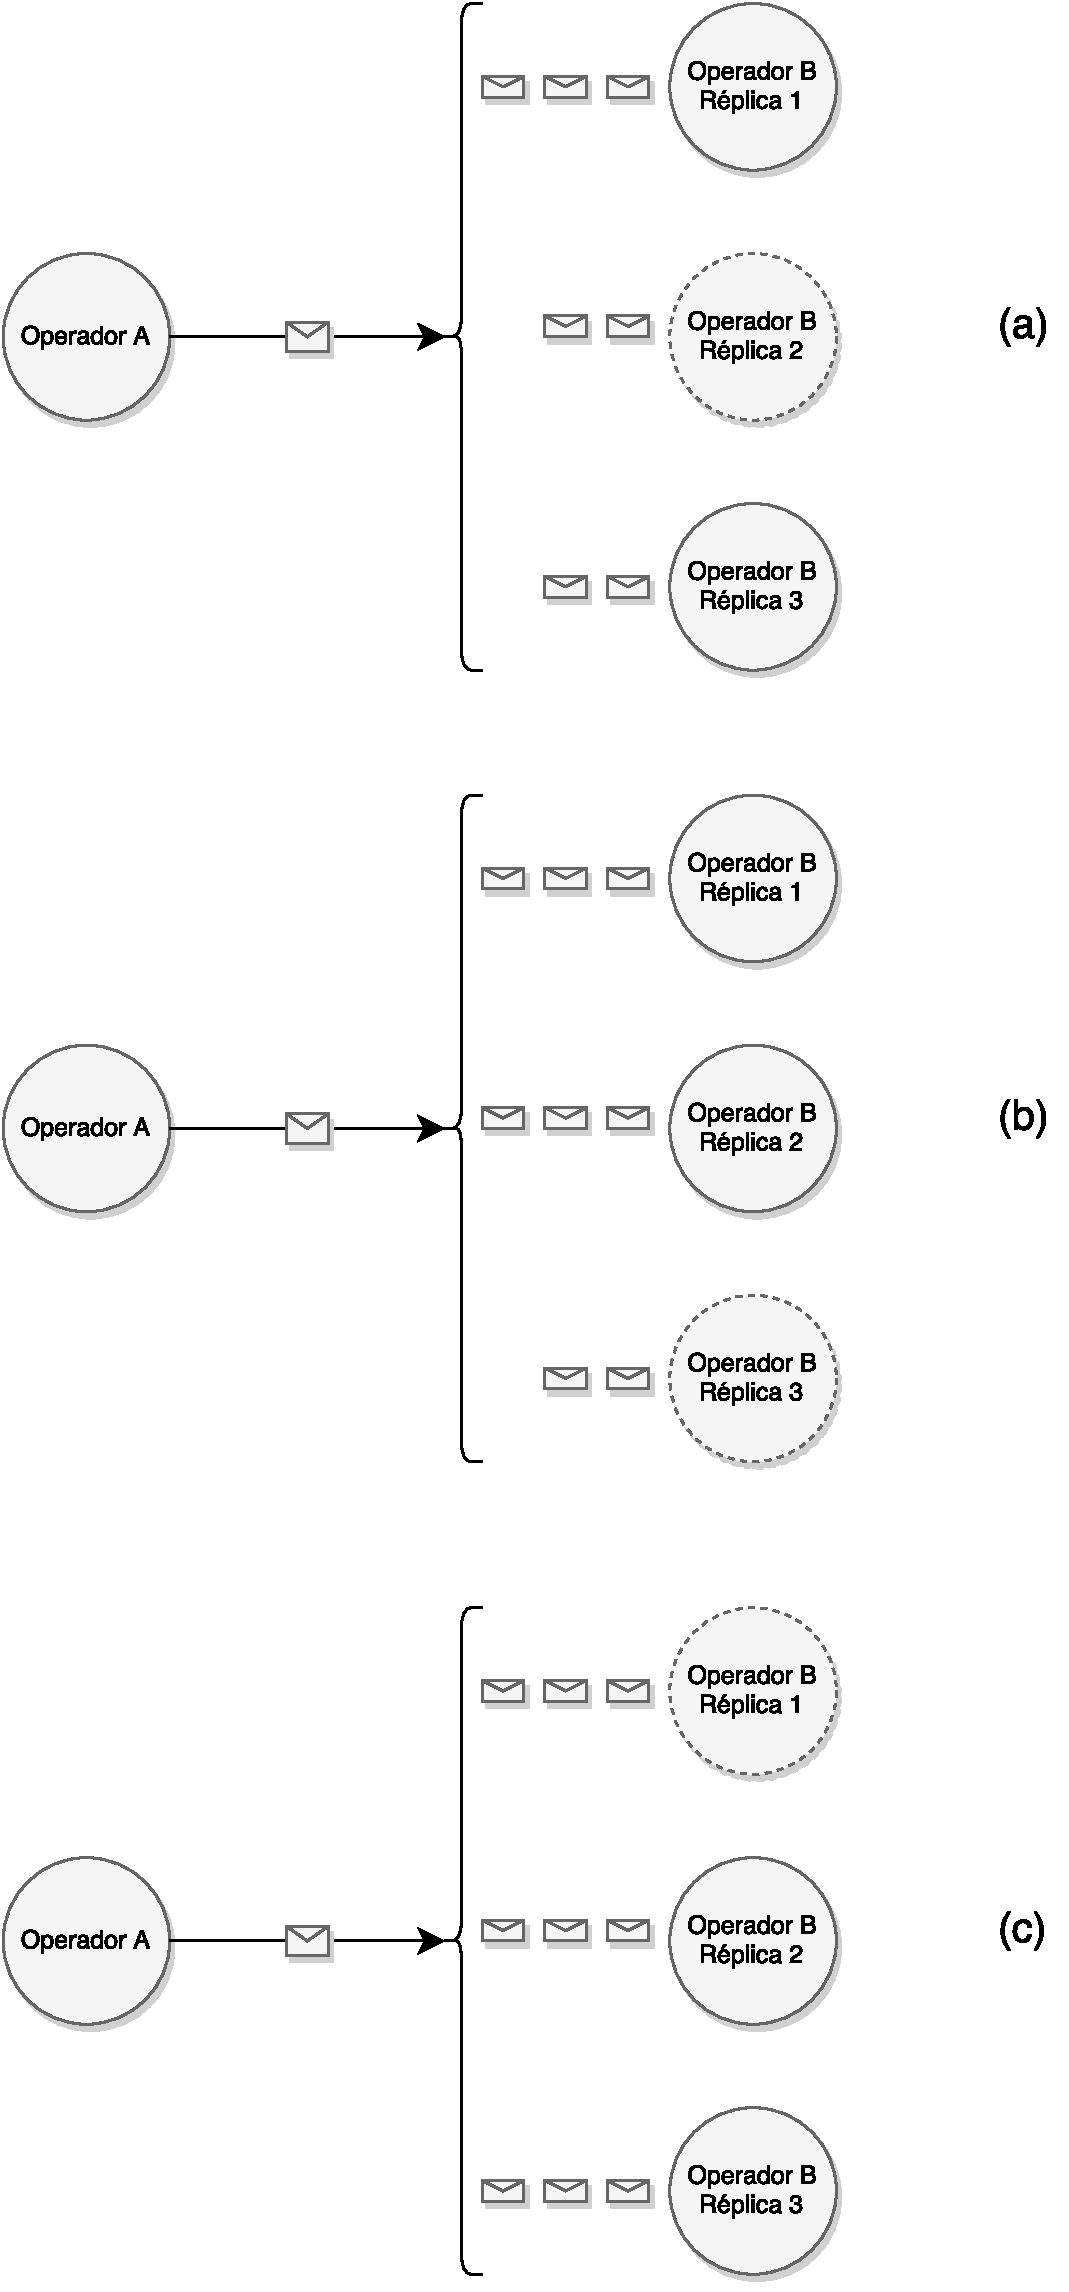
\includegraphics[scale=0.4]{images/DistribucionCarga.pdf}
	\caption{Distribución de la carga entre las réplicas.}
	\label{fig:distCarga}
\end{figure}

%En el Algoritmo \ref{alg:distCarga} se describe la distribución de carga planteada anteriormente, el cual se ha implementado en S4 para ejecutar los experimentos.

%\begin{algorithm}[!ht]
%	\caption{Distribución de carga entre las réplicas de un operador.}
%	\label{alg:distCarga}
%	\begin{algorithmic}[1]
%	\REQUIRE Evento $\epsilon$ y operador $\phi$.
%	\ENSURE Envío del evento a la réplica disponible del operador $\phi$.
%	\STATE $\theta \leftarrow minTamanoCola(\phi)$ \COMMENT Se escoge la réplica que posea menor cola
%	\STATE $envioEvento(\epsilon,\theta$)
%	\end{algorithmic}
%\end{algorithm}

\section{Diseño de los experimentos}
Para los experimentos se han diseñado tres aplicaciones: una que realiza operaciones con estado, otra que realiza operaciones sin estado, y otra aplicación sintética. En el caso que la aplicación posea estado, significa que el operador guarda variables al procesar con el transcurso del tiempo, las cuales son entregadas cada cierto tiempo o al finalizar la ejecución del sistema. Este tipo de aplicaciones son las más utilizadas, dado que utilizan contadores o variables globales, las cuales son necesarias para el análisis de los datos. Un ejemplo de esto, es un sistema que cuenta las palabras de un texto y que envía la cantidad de palabras contadas cada cierto tiempo. Si bien, las aplicaciones sin estado no son tan utilizadas, se consideraron importantes para la validación del modelo, dado que son las aplicaciones más simples y básicas de diseñar y ejecutar. Por otra parte, se ha generado una aplicación sintética, la cual simula el procesamiento de datos por medio de la introducción de retrasos de cada uno de los operadores. Cada operador es una hebra de procesamiento, para reflejar el tiempo de ejecución, por lo que se procede a dormir la hebra por un tiempo predefinido, el cual está determinado por la complejidad del operador. Los operadores más complejos son dormidos por una mayor cantidad de tiempo.

%Se genero una aplicacion sintetica donde se simula el procesamiento de datos por medio de la introduccion de retrasos en cada uno de los operadores. Cada operador es una hebra de procesamiento, para reflejar el tiempo de procesamiento, se procede a dormir la hebra por un tiempo predefinido determinado por la complejidad del operador. Operadores mas complejos serán dormidos una mayor cantidad de tiempo. 

Para la generación del \textit{stream} de la fuente de datos para la primera y segunda aplicación, se ha utilizado un conjunto de 4.5 millones de \textit{tweets}\footnote{Un \textit{tweet} es una publicación o actualización de estado realizada en la red social \textit{Twitter}. Como tal, un \textit{tweet} es un mensaje cuyo límite de extensión son 140 caracteres. Puede contener letras, números, signos y enlaces.}, los cuales fueron recolectados entre los días 27-28 de Febrero y 1-2 de Marzo de 2010, tanto en inglés, portugués y español. Estos contienen información correspondiente a la interacción entre los usuarios durante el terremoto ocurrido el 27 de Febrero en Chile.

Por otra parte, el envío de los datos se ha realizado de dos maneras: constante y variable. El envío de datos constante consiste en enviar 100 eventos por segundo durante todo el experimento. El envío de datos variable consiste en enviar 50 eventos por segundos el primer tercio del experimento, para luego aumentar a 100 eventos por segundo en el segundo tercio, y finalmente, disminuir a 50 eventos por segundos el último tercio de la ejecución.

\subsection{Aplicación 1: Análisis de \textit{tweets} en escenarios de desastres naturales}
La primera aplicación es orientada a un escenario de desastres naturales, donde se genera un grafo que realice un filtrado de palabras, identificación del idioma y conteo de palabras. Ninguno de los operadores posee estado, por lo tanto son independientes. Para la duración de esta prueba se ha considerado un tiempo de ejecución de 70 minutos, \normalsize{cuya duración está basada en el \textit{benchmark} confeccionado por} \citep{ArasuCGMMRST04}. El objetivo de esta aplicación, es comprobar que el sistema diseñado puede funcionar con aplicaciones sin estado, las cuales son las más básicas y sencillas de diseñar en SPS, y que tienen utilidad cuando se hacen análisis directo del flujo de datos.

La aplicación consta del flujo de datos, cuyos datos son la muestra de \textit{tweets} de prueba, y cuatro operadores, los cual son denominados \textit{Stopword}, \textit{Language}, \textit{Counter} y \textit{MongoDB}.

\paragraph{Stopword:} es el operador encargado de leer el \textit{tweet} y remover las palabras que no son relevantes para el análisis de éste, usando una bolsa de palabras (\textit{stopwords}). De esta manera, se puede analizar el texto usando las palabras más representativas de éste y así entregar información más precisa.

\paragraph{Language:} es el operador encargado de identificar el lenguaje existente en el \textit{tweet}, para esto se utilizado una librería \textit{Apache Tika} \citep{mattmann2011tika}. Con ésta se puede realizar un filtro del idioma de los tweets, de tal manera que en caso de ser requerido, sólo continúen los de un idioma en específico, en nuestro caso el español.

\paragraph{Counter:} es el operador encargado de contar la cantidad de palabras que existen en el \textit{tweet} según una bolsa de palabras proporcionada por el programador. Para esta prueba se ha utilizado una bolsa de 26.000 palabras en español. Con esto se pueden detectar los \textit{tweets} que poseen mayor cantidad de palabras claves asociados a una temática o evento en particular.

\paragraph{MongoDB:} es el operador encargado de guardar en la base de datos el evento según los atributos que posee, ya sea por el \textit{tweet} original, sin \textit{stopword}, idioma y cantidad de palabras claves existentes en él. Para esto, se ha utilizado el motor de base de datos no relacional \textit{MongoDB} \citep{chodorow2013mongodb}.

En la Figura \ref{fig:primeraAplicacion} se muestra un ejemplo de la aplicación con sus distintos operadores y relaciones. Las flechas muestran la dirección del flujo de datos emitido por la fuente y los operadores.

\begin{figure}[!hb]
	\centering
		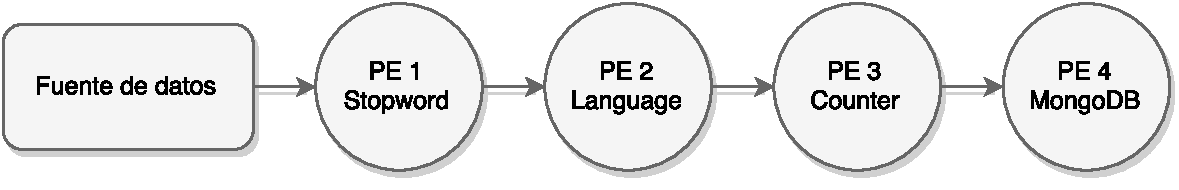
\includegraphics[scale=0.6]{images/App1.pdf}
	\caption{Aplicación 1: Análisis de \textit{tweets} en escenarios de desastres naturales.}
	\label{fig:primeraAplicacion}
\end{figure}

\subsection{Aplicación 2: Contador de palabras en muestras de textos}
La segunda aplicación consiste en un contador de palabras, la cual cuenta la cantidad de veces que se repite una palabra en un conjunto de datos según una bolsa de palabras establecida por el usuario. Esta aplicación se considera con estado, debido que es necesario un contador en el operador, de tal manera de contar la cantidad de veces que se repite cierta palabra según una bolsa de palabras definida. Con esta aplicación es posible analizar posteriormente las palabras más frecuentes emitidas por los usuarios de la red social según un listado de palabras claves. Para la duración de esta prueba se ha considerado un tiempo de 70 minutos, al igual que en la anterior aplicación. El objetivo de esta aplicación es validar el modelo diseñado con aplicaciones con estado, las cuales son las más aplicadas, debido que se realizan análisis generales de los datos, como el caso de los \textit{trending topics} o frecuencia de palabras.

La aplicación consta del flujo de datos, cuyos datos de entrada son la muestra de \textit{tweets} de prueba, y tres operadores, denominados \textit{Split}, \textit{Counter} y \textit{Merge}.

\paragraph{Split:} es el operador encargado de dividir el \textit{tweet}, y enviar un arreglo con las palabras que posee al operador \textit{Counter}.

\paragraph{Counter:} es el operador encargado de llevar las estadísticas de los contadores de cada palabra. Cuando recibe un evento, el operador aumenta el contador de las palabras que corresponde al arreglo de palabras enviado. Las estadísticas son enviadas cada 10 segundos al operador Merge, de tal manera de no enviar flujo constante al siguiente operador y sobrecargar al operador.

\paragraph{Merge:} es el operador encargado de unir las distintas estadísticas enviadas por las distintas réplicas del operador Counter, sumando los valores que corresponde a las palabras enviadas.

En la Figura \ref{fig:segundaAplicacion} se muestra un ejemplo de la segunda aplicación con sus distintos operadores y sus relaciones, de igual manera que en el caso anterior, las flechas reflejan el flujo de datos. Cabe destacar que el único operador que puede replicarse es el \textit{Counter}, debido que el operador \textit{Split} y \textit{Merge} son operadores que soportan la replicación del operador \textit{Counter}, como se explicó en las técnicas de balance de carga en la Sección \ref{sec:fisionBC}.

\begin{figure}[!ht]
	\centering
		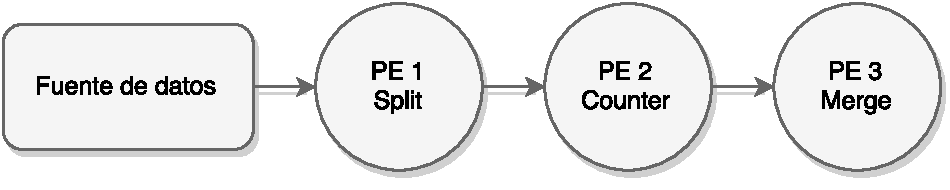
\includegraphics[scale=0.6]{images/App2.pdf}
	\caption{Aplicación 2: Contador de palabras en muestras de textos.}
	\label{fig:segundaAplicacion}
\end{figure}

\subsection{Aplicación 3: Aplicación sintética}
%La tercera aplicación consta de tres operadores sintéticos, los cuales duermen a la hebra asignada al operador un determinado período de tiempo, simulando el tiempo de procesamiento le toma al operador, \normalsize{cuya duración está basada en el \textit{benchmark} confeccionado por} \citep{ArasuCGMMRST04}. El objetivo de este tipo de aplicación, es analizar los costos que posee el sistema implementando.

La tercera aplicación conste de tres operadores sintéticos, los cuales son hebras de procesamiento que llevan a cabo una tarea específica, dependiendo del tipo de operador que representa. Para simular el procesamiento de eventos, se procede a dormir la hebra en el momento que recibe el evento por un tiempo determinado experimental de acuerdo a la complejidad del operador. Esto quiere decir, los operadores más complejos toman mayor tiempo en procesar cada evento, por ende la hebra debe ser dormida un mayor tiempo para simular dicho comportamiento. El objetivo de este experimento es evaluar los costos en términos de memoria y uso de la CPU que posee el modelo elástico propuesto.

%La Tabla \ref{tab:app3-time} muestra el período de tiempo que duerme cada PE \normalsize{la hebra que tiene asignada}. Los tiempos que se han considerado para esta prueba son para generar una sobrecarga en el primer y segundo operador, de tal manera que después afecten al tercer operador. Para la duración de esta prueba se ha considerado un tiempo de 15 minutos.

Para definir los tiempos de procesamientos de las hebras, se crearon operadores reales con complejidades diferentes y midiendo el tiempo que tarda en procesar un evento. Con esto tiempos promedios obtenidos, se ha definido el período de tiempo que duerme la hebra en cada uno de los PEs, los cuales se presentan en la Tabla \ref{tab:app3-time}.

%Para definir los tiempos de procesamiento de las hebras, se crearon operadores reales con complejidades diferentes y se midio el tiempo que tomaba el procesamiento desde que un evento ingresaba al operador hasta que salía procesado. Los tiempos promedios obtenidos para los operadores analizados se presentan en la tabla 5.1

\begin{table}[!ht]
\centering
\caption{Período de tiempo que duerme la hebra asignada al PE.}
\begin{tabular}{| c | c |}
\hline
PE & Tiempo (ms) \\ \hline
1 & 20 \\
2 & 30 \\
3 & 15 \\\hline
\end{tabular}
\label{tab:app3-time}
\end{table}

En la Figura \ref{fig:terceraAplicacion} se muestra un ejemplo de la tercera aplicación con sus distintos operadores y sus relaciones, de igual manera que en los casos anteriores, las flechas reflejan el flujo de datos.

\begin{figure}[!ht]
	\centering
		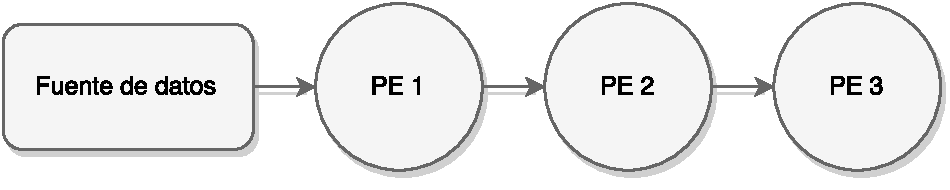
\includegraphics[scale=0.6]{images/App3.pdf}
	\caption{Aplicación 3: Aplicación sintética.}
	\label{fig:terceraAplicacion}
\end{figure}

\section{Evaluación}
Para la ejecución de los experimentos, se ha utilizado un servidor con sistema operativo Ubuntu 14.04.2 LTS, cuyo procesador es un Intel Xeon CPU E5-2650 v2 de 2.60 GHz y con 32 GB de RAM. Cabe recalcar, que el lenguaje de programación es Java, debido a la integración del sistema propuesto en el SPS utilizado. La configuración de S4 es detallada en el Anexo \ref{apendice:config-comm-S4}.

Para la ventana de tiempo del recolector de datos se utiliza un valor de $T_m = 1seg$. Para el administrador de replicas los parámetros del numero de replicas a crear por cada algoritmo se definieron con los valores $\omega = 1$ (reactivo), y $\theta = 5$ (predictivo). Las ventanas de tiempo entre las ejecuciones de los algoritmos son $T_r = 5seg$ y $T_p = 100seg$ respectivamente. Los parámetros del algoritmo predictivo para estos experimentos son una cantidad de muestras de $n = 100$, una cantidad de iteraciones para el cálculo de la distribución estacionaria de $\upsilon = 100000$ y una desviación estándar de $\alpha = 0.25$ entre las variables aleatorias obtenidas por la distribución estacionaria. La cantidad de alertas consecutivas para activar el análisis del algoritmo reactivo es de $\beta = 2$.

\subsection{Aplicación 1: Análisis de \textit{tweets} en escenarios de desastres naturales}
Con la primera aplicación se efectuaron dos experimentos, donde el primero consta de un envío constante de eventos, y el segundo de un envío variable. En ambos experimentos, se han considerado dos pruebas, la primera consiste en la ejecución de la aplicación en un sistema SPS con el uso del modelo elástico, y la segunda sin el uso de éste.

%Para el análisis de los experimentos, se ha considerado la cantidad promdio de eventos procesados en un período, la cantidad total de eventos procesados y las estadísticas de cada PE en el transcurso de la ejecución de la aplicación.

Para el análisis de los experimentos, se ha considerado \normalsize{el rendimiento y la cantidad de réplicas del grafo} y la cantidad total de eventos procesados. \normalsize{En el Anexo} \ref{apendice:estadisticas-operadores} \normalsize{se presentan las estadísticas de cada uno de los operadores.}

%%% EXP1-CONSTANTE OPERADORES %%%

%Las Figuras \ref{fig:app1-uniform-statusStopwordPE-cm} y \ref{fig:app1-uniform-statusStopwordPE-sm} corresponden al primer experimento y muestran las estadísticas del primer operador del grafo, con y sin uso del modelo en la carga de los operadores, respectivamente, ambas con un envío constante de eventos desde la fuente de datos. Se puede observar en el primer gráfico una tasa de llegada ($\lambda$) constante, a diferencia del segundo gráfico, donde varia a partir del segundo 2600.

%El cambio de la tasa de llegada del segundo gráfico se debe a la sobrecarga que existe en el operador, debido que no puede procesar todos los eventos que son enviados a éste, por lo que es un sistema inestable, es decir, $\rho > 1$. Esto genera una acumulación de eventos en el \textit{buffer} del operador, de tal manera que al llenarse, bloquea la recepción de eventos. Por lo que se debe esperar que se liberen eventos del \textit{buffer}, pero como la tasa de rendimiento es baja, al desencolarse, inmediatamente llegada otro evento que vuelve a llenarlo, por lo que la cola se mantiene constante después del segundo 2600. Es por esto mismo que la tasa de llegada disminuye aproximadamente al mismo valor de la tasa de procesamiento.

%Por otra parte, la tasa de rendimiento ($\rho$) graficada en la Figura \ref{fig:app1-uniform-statusStopwordPE-cm} se estabiliza dentro de los primeros 100 segundos, debido que el modelo elástico detecta el operador sobrecargado y lo replica. A diferencia de la Figura \ref{fig:app1-uniform-statusStopwordPE-sm}, en el cual el operador posee una tasa de rendimiento inestable que fluctúa entre 1 y 2, hasta el segundo 2600, donde disminuye debido que la tasa de llegada es menor. Cabe destacar que este operador posee un alto costo computacional, debido que existe una gran cantidad de palabras que debe analizar para cada una de las palabras del \textit{tweet}, por lo que es necesario crear otra réplica.

%En las Figuras \ref{fig:app1-uniform-statusLanguagePE-cm} y \ref{fig:app1-uniform-statusLanguagePE-sm} se observa el siguiente operador de la topología del grafo, el cual no presenta sobrecarga, a excepción del segundo 2400, donde en el caso sin uso del modelo disminuye considerablemente la tasa de procesamiento del PE. Si analizamos las Figuras \ref{fig:app1-uniform-statusStopwordPE-sm} y \ref{fig:app1-uniform-statusLanguagePE-sm}, empiezan aproximadamente desde el rango de tiempo (2400s, 2600s) los problemas de procesamiento de los operadores, por lo tanto, se puede deducir que si el problema surge en un operador no es un problema aislado, sino que también influye a los siguientes operadores.

%Se puede observar como con el transcurso de los primeros 100 segundos en la Figura \ref{fig:app1-uniform-statusCounterPE-cm}, aumenta la cantidad de réplicas hasta llegar a 5, el cual es su óptimo, para ir procesando la cantidad de eventos actuales y disminuir la cola existente en el sistema. Esto en contraposición a la Figura \ref{fig:app1-uniform-statusCounterPE-sm}, donde la inexistencia de replicación, genera una cola la cual se mantiene constante en el segundo 2400.

%Finalmente, se encuentra el último operador, el cual no presenta grandes problemas de procesamiento tanto en las Figuras \ref{fig:app1-uniform-statusMongoPE-cm} y \ref{fig:app1-uniform-statusMongoPE-sm}. Esto se debe a que el tiempo de procesamiento es bajo y nunca llega una cantidad de eventos considerable para provocar una sobrecarga. Además, es importante destacar que en la Figura \ref{fig:app1-uniform-statusMongoPE-sm} se registra una menor tasa de llegada, con un promedio de $83\%$ menos de eventos que un SPS ejecutado con el modelo elástico.

%\begin{figure}[p]
%\centering
%    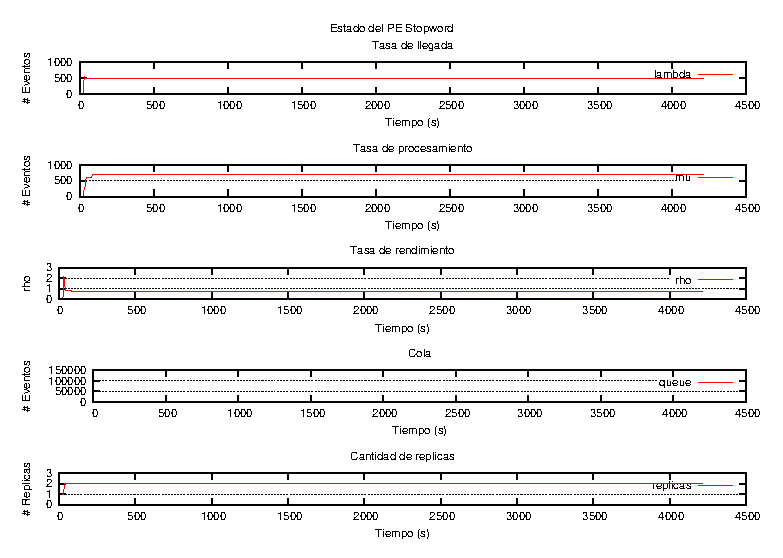
\includegraphics[scale=1.1]{images/exp/app1/uniform/cm/statusStopwordPE.eps}
%    \caption{Estadísticas del PE Stopword en la primera aplicación con un envío constante de la fuente de datos con uso del modelo.}
%    \label{fig:app1-uniform-statusStopwordPE-cm}
%\end{figure}
%
%\begin{figure}[p]
%\centering
%    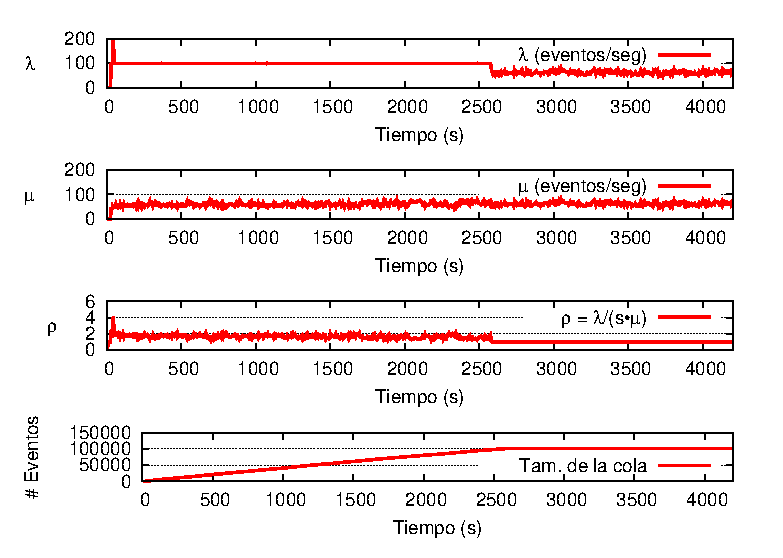
\includegraphics[scale=1.1]{images/exp/app1/uniform/sm/statusStopwordPE.eps}
%    \caption{Estadísticas del PE Stopword en la primera aplicación con un envío constante de la fuente de datos sin uso del modelo.}
%    \label{fig:app1-uniform-statusStopwordPE-sm}
%\end{figure}
%
%\begin{figure}[p]
%\centering
%    \includegraphics[scale=1.1]{images/exp/app1/uniform/cm/statusLanguagePE.eps}
%    \caption{Estadísticas del PE Language en la primera aplicación con un envío constante de la fuente de datos con uso del modelo.}
%    \label{fig:app1-uniform-statusLanguagePE-cm}
%\end{figure}
%
%\begin{figure}[p]
%\centering
%    \includegraphics[scale=1.1]{images/exp/app1/uniform/sm/statusLanguagePE.eps}
%    \caption{Estadísticas del PE Language en la primera aplicación con un envío constante de la fuente de datos sin uso del modelo.}
%    \label{fig:app1-uniform-statusLanguagePE-sm}
%\end{figure}
%
%\begin{figure}[p]
%\centering
%    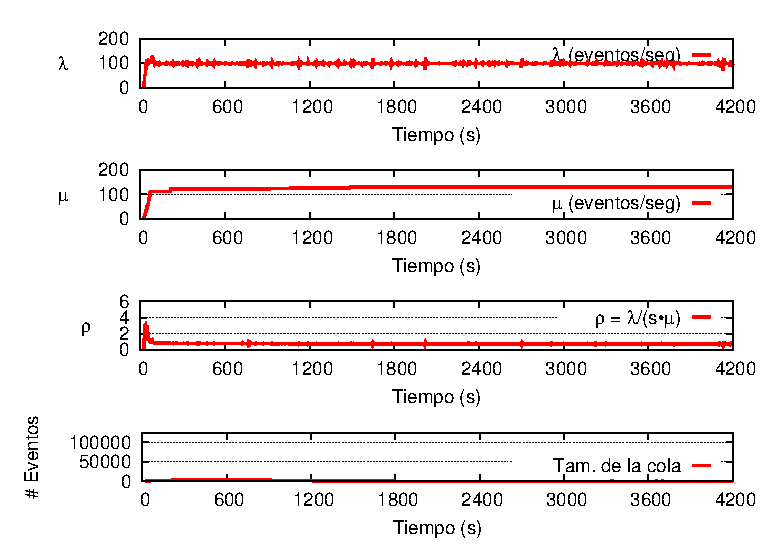
\includegraphics[scale=1.1]{images/exp/app1/uniform/cm/statusCounterPE.eps}
%    \caption{Estadísticas del PE Counter en la primera aplicación con un envío constante de la fuente de datos con uso del modelo.}
%    \label{fig:app1-uniform-statusCounterPE-cm}
%\end{figure}
%
%\begin{figure}[p]
%\centering
%    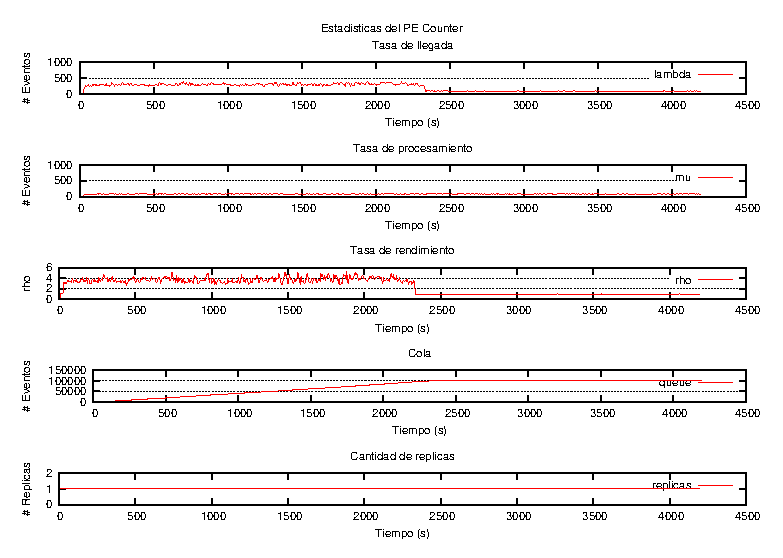
\includegraphics[scale=1.1]{images/exp/app1/uniform/sm/statusCounterPE.eps}
%    \caption{Estadísticas del PE Counter en la primera aplicación con un envío constante de la fuente de datos sin uso del modelo.}
%    \label{fig:app1-uniform-statusCounterPE-sm}
%\end{figure}
%
%\begin{figure}[p]
%\centering
%    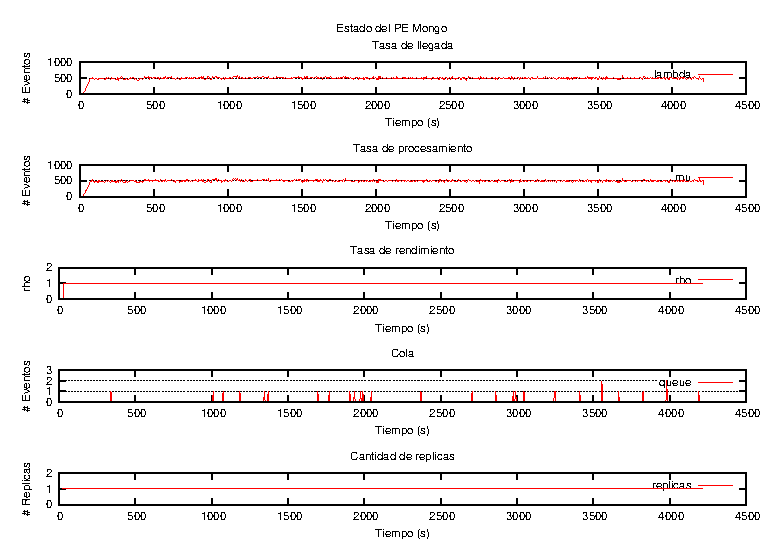
\includegraphics[scale=1.1]{images/exp/app1/uniform/cm/statusMongoPE.eps}
%    \caption{Estadísticas del PE Mongo en la primera aplicación con un envío constante de la fuente de datos con uso del modelo.}
%    \label{fig:app1-uniform-statusMongoPE-cm}
%\end{figure}
%
%\begin{figure}[p]
%\centering
%    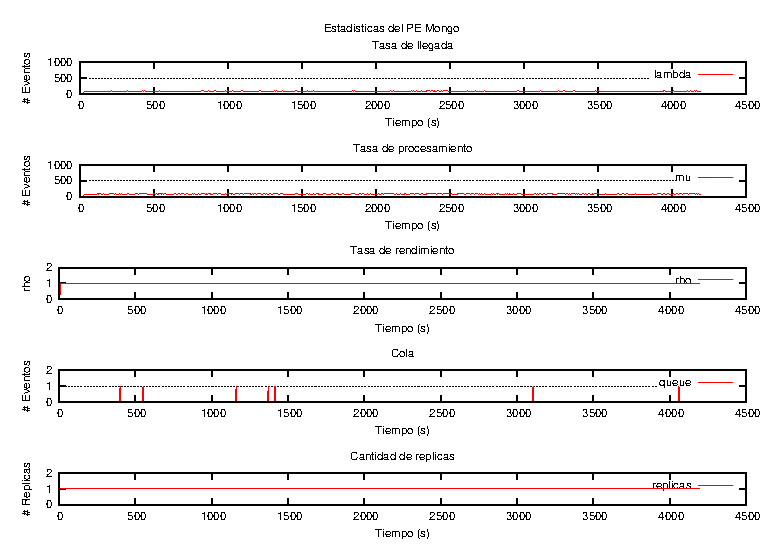
\includegraphics[scale=1.1]{images/exp/app1/uniform/sm/statusMongoPE.eps}
%    \caption{Estadísticas del PE Mongo en la primera aplicación con un envío constante de la fuente de datos sin uso del modelo.}
%    \label{fig:app1-uniform-statusMongoPE-sm}
%\end{figure}

%%% EXP1-CONSTANTE PERFORMANCE %%%

Las Figuras \ref{fig:app1-uniform-processSystem-cm} y \ref{fig:app1-uniform-processSystem-sm} \normalsize{corresponden al primer experimento y muestra el rendimiento que posee el sistema, y como varía la cantidad de réplicas totales del grafo según el flujo constante de datos.} En la Figura \ref{fig:app1-uniform-processSystem-cm} \normalsize{se observa que en los primero segundos existe una sobrecarga en el grafo, específicamente en los PE Stopword y Counter, por lo que el modelo detecta esta inestabilidad en el sistema y aumenta la cantidad de réplicas de los operadores} (véase Anexo \ref{apendice:estadisticas-operadores}), \normalsize{logrando un procesamiento promedio de  98 eventos por segundo.} En el caso de la Figura \ref{fig:app1-uniform-processSystem-sm} \normalsize{no existe un aumento en la cantidad de réplicas, por lo tanto, no existe un aumento de la cantidad de datos procesados, alcanzando un promedio de 16 eventos procesados por segundo. Se puede observar que en esta figura en el segundo 2600 la tasa de entrada disminuye considerablemente, esto es resultado de la sobrecarga del sistema. Comparando ambos escenarios se puede observar que la utilización del modelo elástico para esta aplicación ha logrado mejorar el rendimiento del sistema, logrando incrementar 5 veces el numero total de eventos procesados.}

\begin{figure}[!ht]
	\centering
	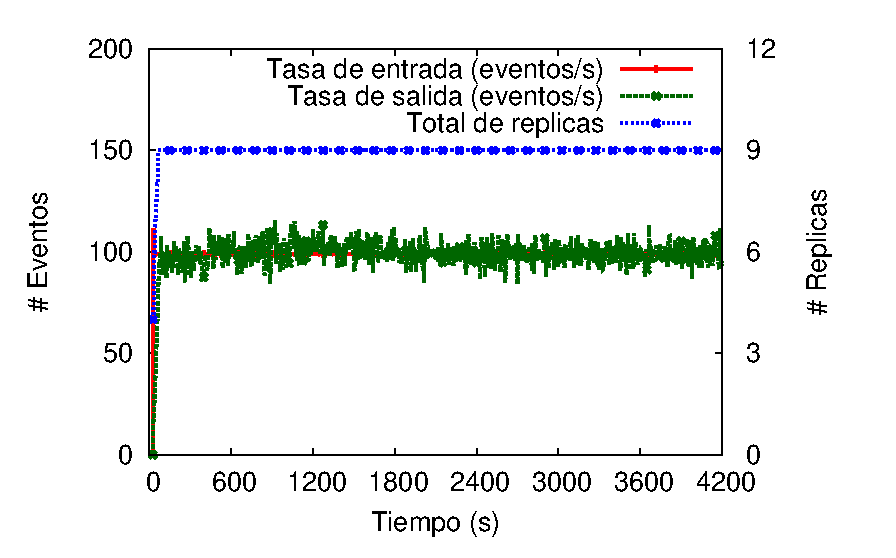
\includegraphics[scale=0.65]{images/exp/app1/uniform/cm/processSystem.eps}
    \caption{Rendimiento y cantidad de réplicas totales del grafo en la primera aplicación con envío constante de la fuente de datos con uso del modelo.}
	\label{fig:app1-uniform-processSystem-cm}
\end{figure}

\begin{figure}[!ht]
	\centering
	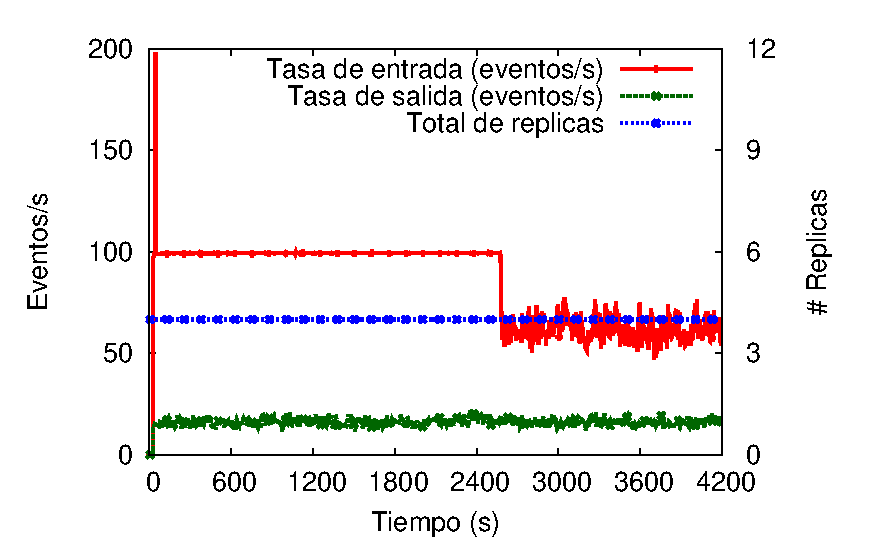
\includegraphics[scale=0.65]{images/exp/app1/uniform/sm/processSystem.eps}
    \caption{Rendimiento y cantidad de réplicas totales del grafo en la primera aplicación con envío constante de la fuente de datos sin uso del modelo.}
	\label{fig:app1-uniform-processSystem-sm}
\end{figure}

%%% EXP1-CONSTANTE CANT. PROMEDIO EVENTOS PROCESADOS %%%

% Por otra parte, también se ha analizado la cantidad promedio de eventos procesados en cada período la cual es presentada en las Figuras \ref{fig:app1-uniform-cm-avgEventProcess} y \ref{fig:app1-uniform-sm-avgEventProcess}. Como se puede apreciar en el primero gráfico, en los primeros 50 segundos se observa una mejora considerable en la cantidad de eventos procesados, donde posteriormente se procesan aproximadamente 480 eventos por período en el sistema con modelo, a diferencia del SPS sin uso del modelo, que procesa 90 eventos por período aproximadamente, alcanzando a procesar 5 veces más eventos con el modelo. Esta mejora se debe a la replicación de los operadores que poseen mayor sobrecarga, por lo que al aumentar la cantidad de réplicas, aumenta la tasa de procesamiento, lo que significa mayor cantidad de flujo para el próximo operador.

%\begin{figure}[ht]
%\centering
%
%\begin{minipage}[c]{0.45\textwidth}
%\centering
%    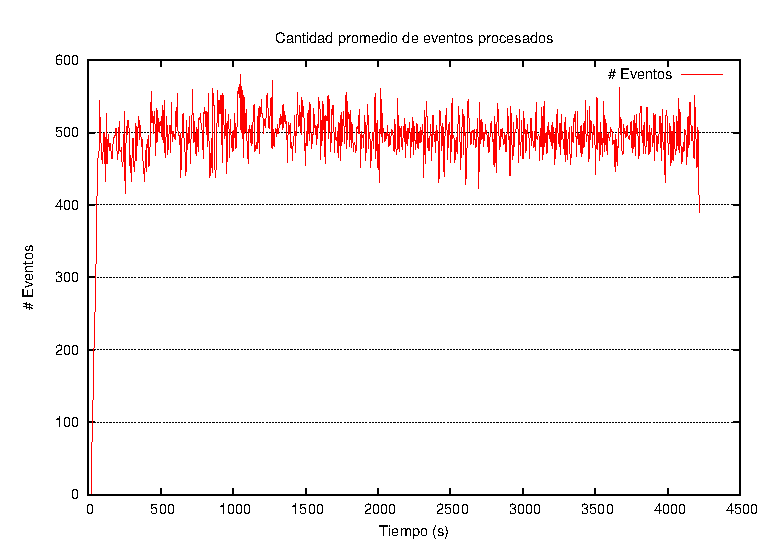
\includegraphics[width=\textwidth]{images/exp/app1/uniform/cm/avgEventProcess.eps}
%    \caption{Cantidad promedio de eventos procesados en cada período en la primera aplicación con un envío constante de la fuente de datos con uso del modelo.}
%    \label{fig:app1-uniform-cm-avgEventProcess}
%\end{minipage} \hspace*{1cm}
%\begin{minipage}[c]{0.45\textwidth}
%\centering
%    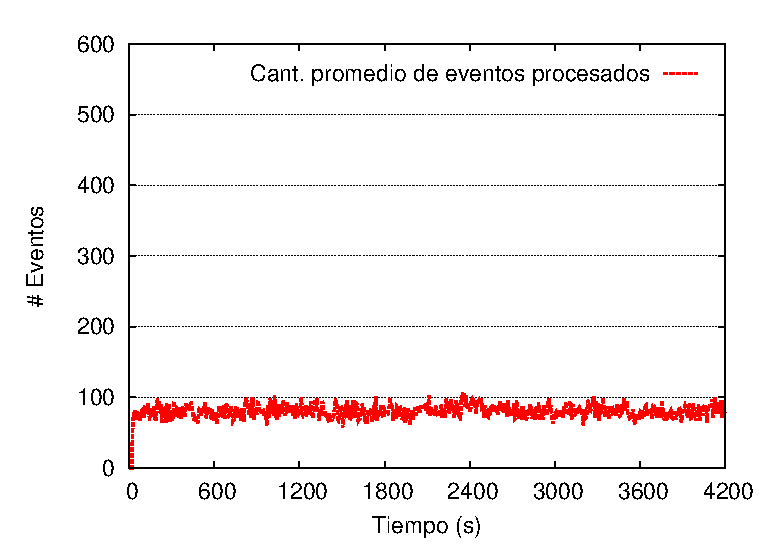
\includegraphics[width=\textwidth]{images/exp/app1/uniform/sm/avgEventProcess.eps}
%    \caption{Cantidad promedio de eventos procesados en cada período en la primera aplicación con un envío constante de la fuente de datos sin uso del modelo.}
%    \label{fig:app1-uniform-sm-avgEventProcess}
%\end{minipage}
%
%\end{figure}

%%% EXP1-CONSTANTE EVENTOS TOTALES PROCESADOS %%%
En las Figuras \ref{fig:app1-uniform-eventCount-cm} y \ref{fig:app1-uniform-eventCount-sm} se presenta la cantidad total de eventos procesados en el transcurso de la ejecución en cada uno de los operadores, con y sin uso del modelo respectivamente. En el primer gráfico los cuatro operadores del SPS van aumentando la cantidad total de eventos procesados linealmente y con la misma pendiente, tan sólo existe una menor cantidad de eventos procesados en el tercer PE, lo cual se traslada al cuarto PE, debido a que al procesar menor cantidad de eventos en el tercer PE, llega una menor cantidad de eventos al cuarto PE. En este gráfico se alcanza un total de 401.618 eventos procesados. En cambio, en el segundo gráfico las curvas de cantidad de eventos procesados son muy distintas entre los distintos operadores, lo cual se ve reflejado desde la cantidad de eventos procesados en el primer operador hasta la cantidad total de eventos procesados por el sistema, el que alcanza un total de 67.141 eventos. Por lo que con el uso del modelo elástico se ha procesado 6 veces más eventos que los procesados durante el mismo período de tiempo sin el uso de éste.

\begin{figure}[!ht]
	\centering
    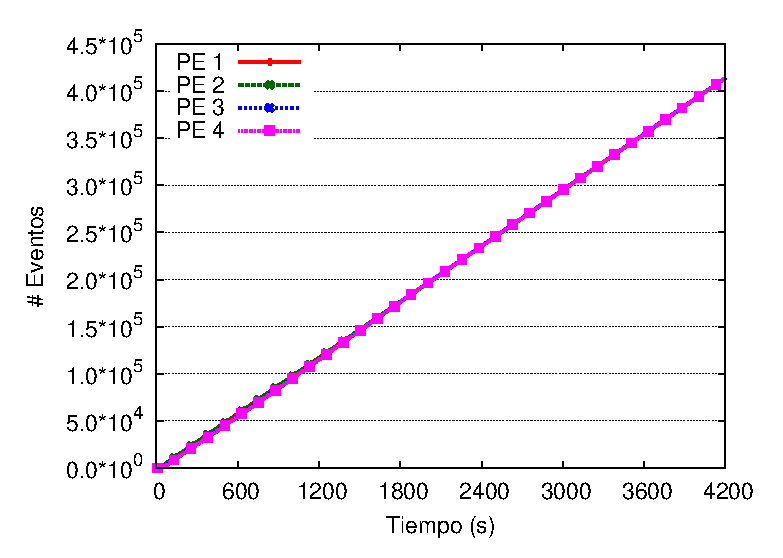
\includegraphics[scale=0.7]{images/exp/app1/uniform/cm/eventCount.eps}
    \caption{Cantidad total de eventos procesados en la primera aplicación con un envío constante de la fuente de datos con uso del modelo.}
    \label{fig:app1-uniform-eventCount-cm}
\end{figure}

\begin{figure}[!ht]
	\centering
    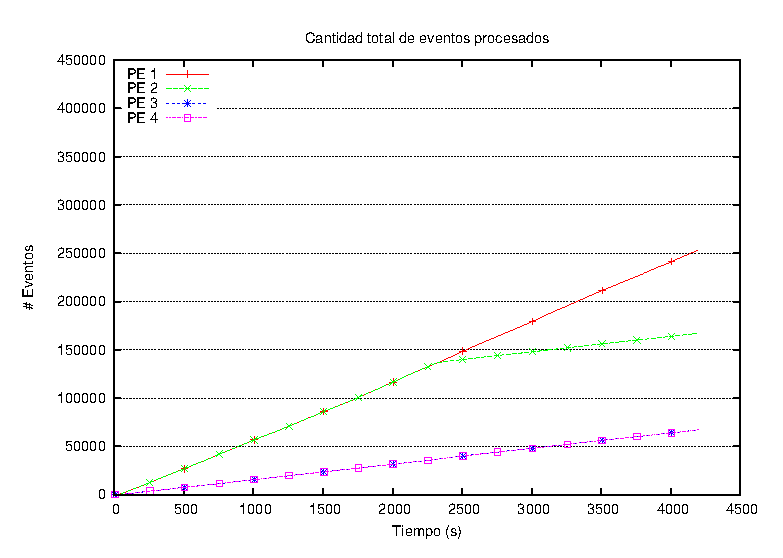
\includegraphics[scale=0.7]{images/exp/app1/uniform/sm/eventCount.eps}
    \caption{Cantidad total de eventos procesados en la primera aplicación con un envío constante de la fuente de datos sin uso del modelo.}
    \label{fig:app1-uniform-eventCount-sm}
\end{figure}

%%% EXP1-VARIABLE OPERADORES %%%

%En el segundo experimento se observa que en las Figuras \ref{fig:app1-normal-statusStopwordPE-cm} y \ref{fig:app1-normal-statusStopwordPE-sm}, se muestra el comportamiento del primer operador con un envío variable de la fuente de datos. En las estadísticas se aprecia que existe un comportamiento estable hasta el segundo 1100, con y sin uso del modelo. Esto se debe a que el operador no posee gran cantidad de demanda dada la tasa de llegada, la cual varía en el segundo 1100, debido al aumento de la cantidad de eventos entrantes. Esto implica que el operador debe procesar mayor cantidad de datos, aumentando así la cantidad de réplicas del mismo. Luego en el segundo 3200 disminuye la tasa de llegada, por lo que la tasa de rendimiento vuelve a ser estable en el sistema con y sin modelo, ya que es menor la cantidad de eventos que deben ser procesados, lo que significa también la disminución de una réplica en el sistema con uso del modelo.
%
%El comportamiento variable del flujo de entrada sólo se puede apreciar con mayor detalle en el primer operador cuando no se usa el modelo, debido que la tasa de llegada del segundo depende de la tasa de procesamiento del primero, y como no existe un aumento de la tasa de procesamiento, sólo aumenta hasta lo que puede procesar con un sólo operador.
%
%En las Figuras \ref{fig:app1-normal-statusLanguagePE-cm} y \ref{fig:app1-normal-statusLanguagePE-sm} se observa la diferencia entre las tasas de llegada, debido a que en el primer gráfico, existe una variación de la tasa de llegada, dado el uso del modelo elástico. Esto se debe a que el primer operador no procesa todos los eventos entrantes, e implica que la tasa de llegada es constante en el segundo operador. Independiente del uso o no del modelo, no existe una sobrecarga en el operador, por lo que el comportamiento del operador siempre es estable.
%
%Luego, en las Figuras \ref{fig:app1-normal-statusCounterPE-cm} y \ref{fig:app1-normal-statusCounterPE-sm} se presenta el tercer operador, en el cual existe una sobrecarga desde el inicio del sistema. Esto se debe a la gran cantidad de palabras que debe comparar, por lo que al realizar la iteración para verificar si existe o no una palabra, requiere un alto costo computacional. En el primer gráfico se puede analizar que en los primeros 100 segundos, el operador aumenta a trusandoes réplicas, estabilizándose el rendimiento del mismo. En cambio, en el sistema sin el uso del modelo elástico existe una tasa de procesamiento constante, por lo que la tasa de rendimiento es inestable en el transcurso de todo el experimento. También se muestra una disminución en la cantidad de réplicas en el segundo 3200, y esto se debe a que la cantidad de réplicas necesarias para el sistema es menor, dado que el envío de datos de la fuente de datos ha disminuido, y por ende la tasa de llegada del PE también.
%
%Dentro de los análisis importantes que se pueden realizar al gráfico de la Figura \ref{fig:app1-normal-statusCounterPE-cm}, es que en el primer tercio de la prueba con uso del modelo, la cantidad óptima de operadores fue 4, pero en el último tercio fue de 5, siendo que ambos poseen la misma tasa de llegada. Esto se debe a que al existir 7 réplicas en el segundo tercio y disminuir la tasa de llegada, se detectaron operadores ociosos. Dado que el $\rho$ del operador es menor a 0.5, por lo tanto para encontrarse a un estado estable, es necesario converger a 0.5, por lo que al estabilizarse el operador, su $\rho$ tiende a estar más cerca de 0.5 que de 1. De esta manera, las tasas de rendimiento son distintas en el primer y último tercio, por lo que puede darse que las réplicas del primer tercio sea mayor que el último tercio.
%
%Por último, en el cuarto operador se puede apreciar en las Figuras \ref{fig:app1-normal-statusMongoPE-cm} y \ref{fig:app1-normal-statusMongoPE-sm} su comportamiento con y sin uso del modelo elástico respectivamente. En ambos casos se muestra una tasa de rendimiento estable, la diferencia está en la tasa de llegada que posee cada uno de los sistemas, donde en el primer gráfico la tasa de llegada es variable, y en el segundo es constante, por lo que existe una menor tasa de rendimiento, lo que significa una menor cantidad de eventos procesados.

%\begin{figure}[p]
%\centering
%    \includegraphics[scale=1.1]{images/exp/app1/normal/cm/statusStopwordPE.eps}
%    \caption{Estadísticas del PE Stopword en la primera aplicación con un envío variable de la fuente de datos con uso del modelo.}
%    \label{fig:app1-normal-statusStopwordPE-cm}
%\end{figure}
%
%\begin{figure}[p]
%\centering
%    \includegraphics[scale=1.1]{images/exp/app1/normal/sm/statusStopwordPE.eps}
%    \caption{Estadísticas del PE Stopword en la primera aplicación con un envío variable de la fuente de datos sin uso del modelo.}
%    \label{fig:app1-normal-statusStopwordPE-sm}
%\end{figure}
%
%\begin{figure}[p]
%\centering
%    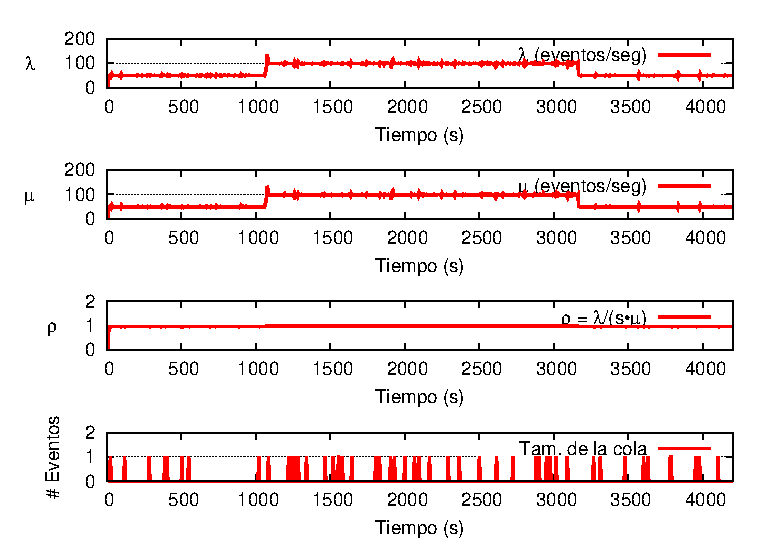
\includegraphics[scale=1.1]{images/exp/app1/normal/cm/statusLanguagePE.eps}
%    \caption{Estadísticas del PE Language en la primera aplicación con un envío variable de la fuente de datos con uso del modelo.}
%    \label{fig:app1-normal-statusLanguagePE-cm}
%\end{figure}
%
%\begin{figure}[p]
%\centering
%    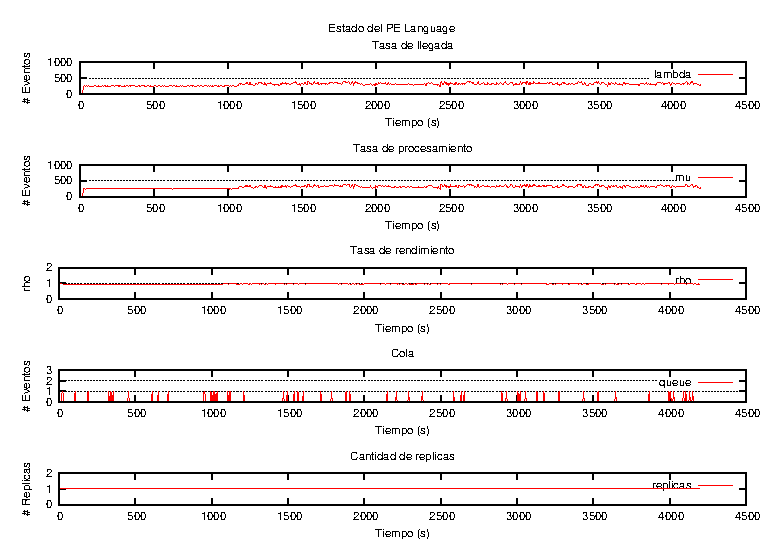
\includegraphics[scale=1.1]{images/exp/app1/normal/sm/statusLanguagePE.eps}
%    \caption{Estadísticas del PE Language en la primera aplicación con un envío variable de la fuente de datos sin uso del modelo.}
%    \label{fig:app1-normal-statusLanguagePE-sm}
%\end{figure}
%
%\begin{figure}[p]
%\centering
%    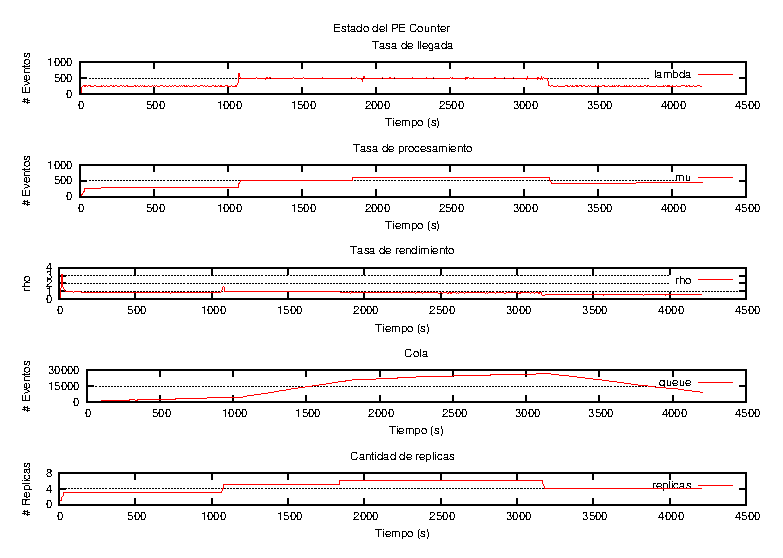
\includegraphics[scale=1.1]{images/exp/app1/normal/cm/statusCounterPE.eps}
%    \caption{Estadísticas del PE Counter en la primera aplicación con un envío variable de la fuente de datos con uso del modelo.}
%    \label{fig:app1-normal-statusCounterPE-cm}
%\end{figure}
%
%\begin{figure}[p]
%\centering
%    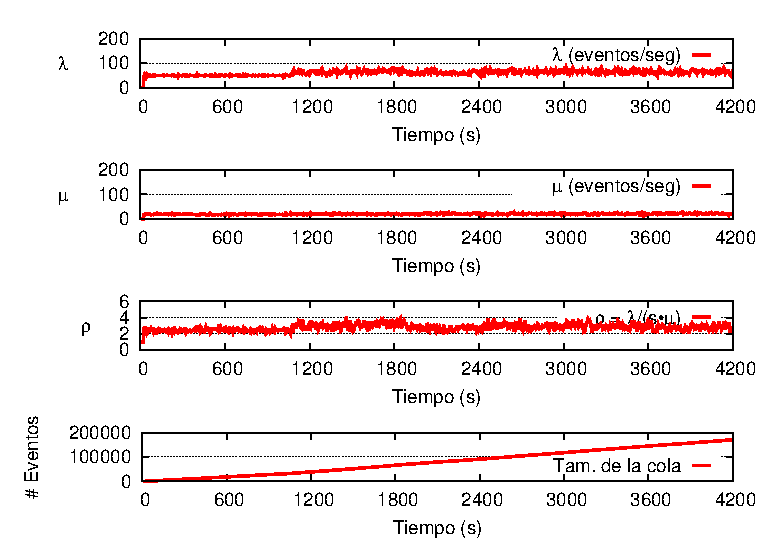
\includegraphics[scale=1.1]{images/exp/app1/normal/sm/statusCounterPE.eps}
%    \caption{Estadísticas del PE Counter en la primera aplicación con un envío variable de la fuente de datos sin uso del modelo.}
%    \label{fig:app1-normal-statusCounterPE-sm}
%\end{figure}
%
%\begin{figure}[p]
%\centering
%    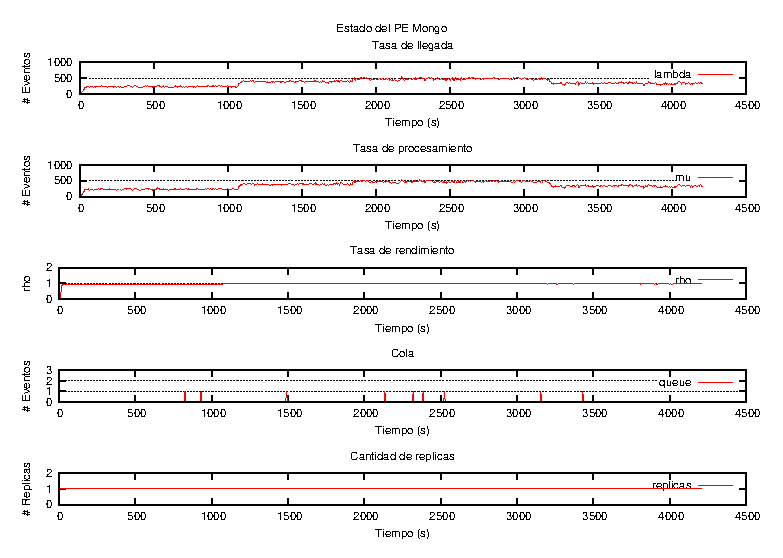
\includegraphics[scale=1.1]{images/exp/app1/normal/cm/statusMongoPE.eps}
%    \caption{Estadísticas del PE Mongo en la primera aplicación con un envío variable de la fuente de datos con uso del modelo.}
%    \label{fig:app1-normal-statusMongoPE-cm}
%\end{figure}
%
%\begin{figure}[p]
%\centering
%    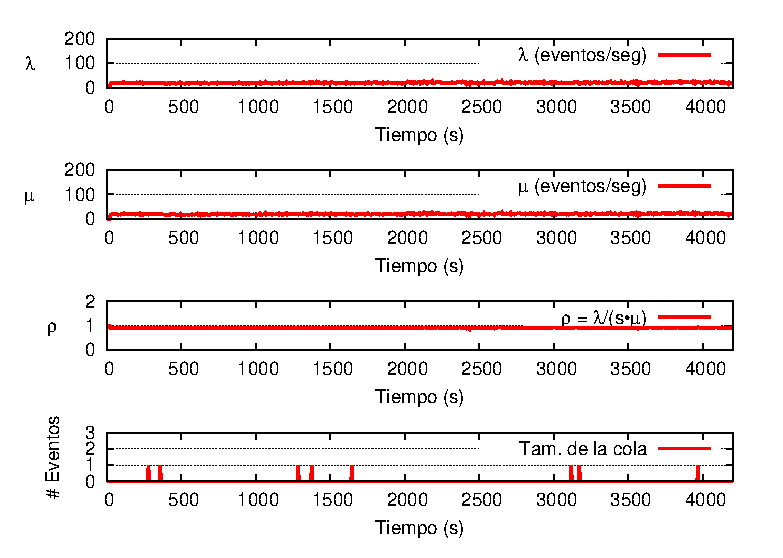
\includegraphics[scale=1.1]{images/exp/app1/normal/sm/statusMongoPE.eps}
%    \caption{Estadísticas del PE Mongo en la primera aplicación con un envío variable de la fuente de datos sin uso del modelo.}
%    \label{fig:app1-normal-statusMongoPE-sm}
%\end{figure}

%%% EXP1-VARIABLE CANT. PROMEDIO DE EVENTOS %%%

%Como se ha expuesto anteriormente, la cantidad de datos procesados en el sistema sin uso del modelo es menor, y esto se puede apreciar en la cantidad promedio de eventos procesados en cada período con y sin uso del modelo, como se muestra en las Figuras \ref{fig:app1-normal-cm-avgEventProcess} y \ref{fig:app1-normal-sm-avgEventProcess} respectivamente. En el primer gráfico existe un promedio de 225 eventos por período, el cual aumenta a un promedio de 438 eventos por período en el segundo 1100, a raíz de un aumento del flujo de la fuente de datos, para que luego disminuya a un promedio de 332 eventos por período en el segundo 3200, debido a la disminución del flujo. En cambio, en el segundo gráfico la cantidad promedio de eventos procesados es constante, debido que no existe optimización alguna en el sistema, por lo que en todo el experimento se procesan 98 eventos por período aproximadamente. Dado esto, en el primer tramo existe una mejora de 2 veces más eventos, luego en el segundo tramo una mejora de 4 veces más, y por último, tercer tramo una mejora de 3 veces más.

%\begin{figure}[!ht]
%\centering
%
%\begin{minipage}[c]{0.45\textwidth}
%\centering
%    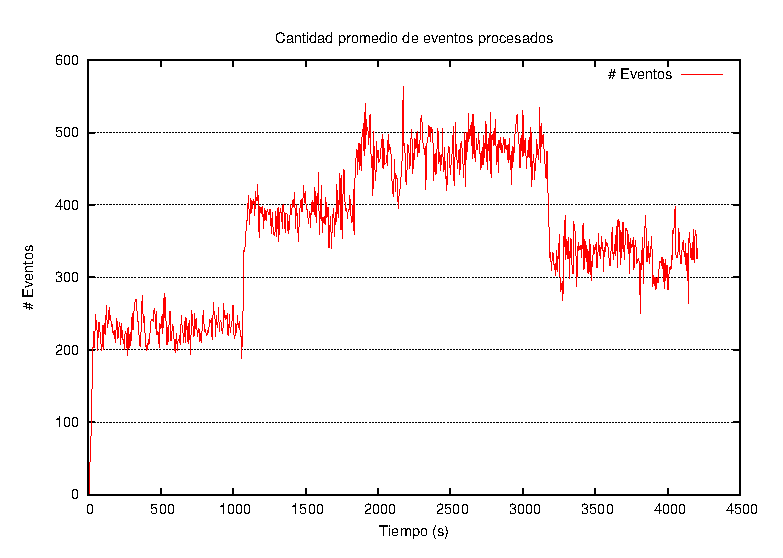
\includegraphics[width=\textwidth]{images/exp/app1/normal/cm/avgEventProcess.eps}
%    \caption{Cantidad promedio de eventos procesados en cada período en la primera aplicación con un envío variable de la fuente de datos con uso del modelo.}
%    \label{fig:app1-normal-cm-avgEventProcess}
%\end{minipage}
%\hspace*{1cm}
%\begin{minipage}[c]{0.45\textwidth}
%\centering
%    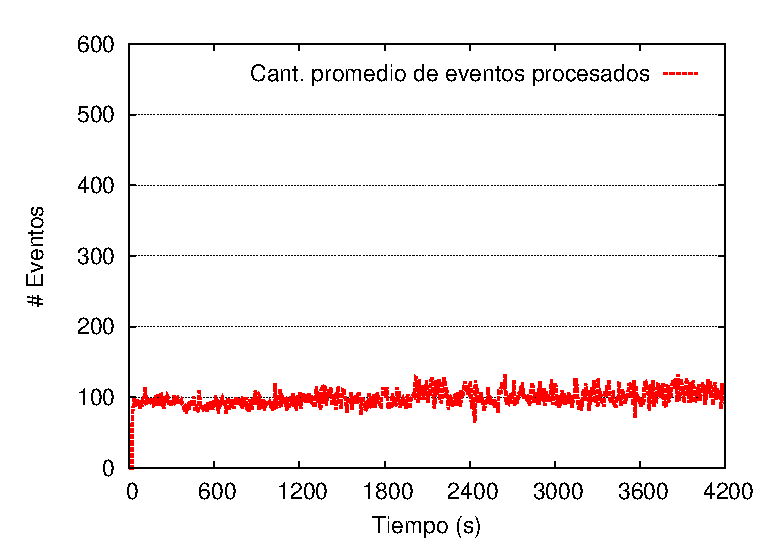
\includegraphics[width=\textwidth]{images/exp/app1/normal/sm/avgEventProcess.eps}
%    \caption{Cantidad promedio de eventos procesados en cada período en la primera aplicación con un envío variable de la fuente de datos sin uso del modelo.}
%    \label{fig:app1-normal-sm-avgEventProcess}
%\end{minipage}
%
%\end{figure}

%%% EXP1-VARIABLE PERFORMANCE %%%
Las Figuras \ref{fig:app1-normal-processSystem-cm} y \ref{fig:app1-normal-processSystem-sm} \normalsize{corresponden al segundo experimento y muestra el rendimiento que posee el sistema, y como varía la cantidad de réplicas totales del grafo según el flujo de datos.} En la Figura \ref{fig:app1-normal-processSystem-cm} \normalsize{se muestra como el sistema fue adaptando la cantidad de réplicas según la tasa de entrada, de tal manera de modificar la cantidad de réplicas según la necesidad que se posea. Por ejemplo, en el primer y segundo tercio aumenta la cantidad de réplicas, no así en el último, donde disminuye la cantidad de réplicas, debido que existe un exceso en la cantidad de recursos. El promedio en la tasa de salida en esta prueba es de 72 eventos por segundo.} Por otra parte, en la Figura \ref{fig:app1-normal-processSystem-sm} \normalsize{existe una tasa de salida constante, lo cual refleja la nula adaptabilidad del sistema según el flujo entrante, habiendo un promedio de 19 eventos procesados por segundo. De los resultados presentados, se puede observar una clara mejora en el rendimiento, alcanzado a procesar hasta 3 veces más eventos que la versión sin el modelo elástico.}

\begin{figure}[!ht]
	\centering
	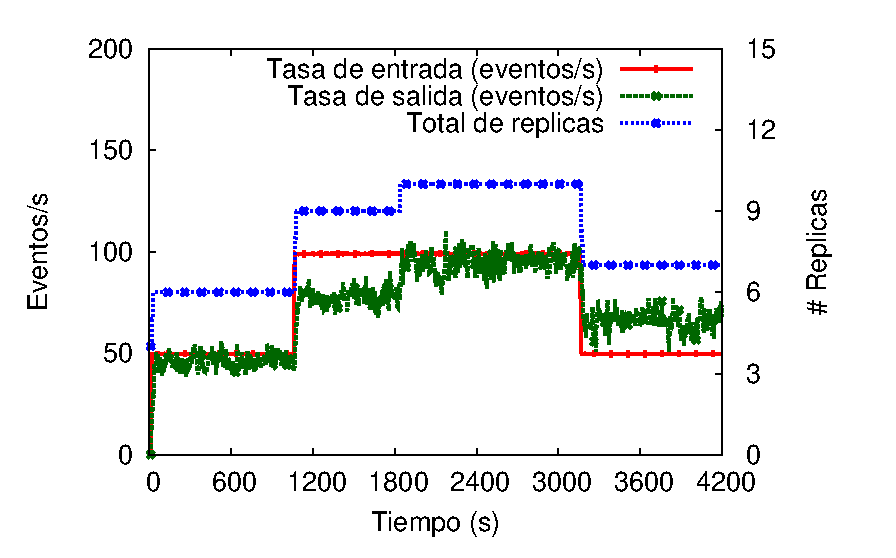
\includegraphics[scale=0.7]{images/exp/app1/normal/cm/processSystem.eps}
    \caption{Rendimiento y cantidad de réplicas totales del grafo en la primera aplicación con envío variable de la fuente de datos con uso del modelo.}
	\label{fig:app1-normal-processSystem-cm}
\end{figure}

\begin{figure}[!ht]
	\centering
	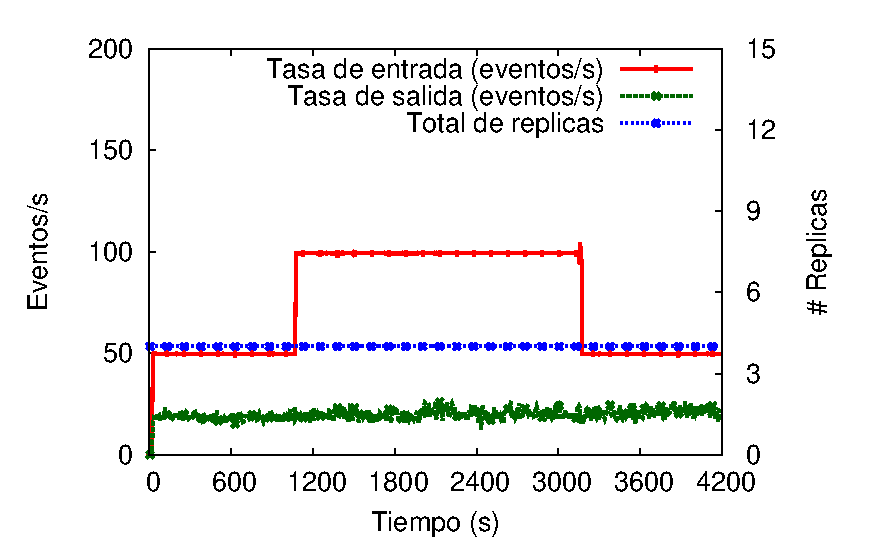
\includegraphics[scale=0.7]{images/exp/app1/normal/sm/processSystem.eps}
    \caption{Rendimiento y cantidad de réplicas totales del grafo en la primera aplicación con envío variable de la fuente de datos sin uso del modelo.}
	\label{fig:app1-normal-processSystem-sm}
\end{figure}

%%% EXP1-VARIABLE EVENTOS TOTALES %%%
Por otra parte, la cantidad total de eventos procesados en el experimento, se observa en las Figuras \ref{fig:app1-normal-eventCount-cm} y \ref{fig:app1-normal-eventCount-sm} con y sin uso del modelo respectivamente. En el primer gráfico se observa variaciones en la curva en el segundo 1100 y 3200, lo cual son los segundos en los cuales hubo un cambio en el flujo de la fuente de datos, por lo que aumenta y disminuye respectivamente la tasa de llegada. En cambio, en el segundo gráfico no se aprecia esto, debido que independiente de la tasa de llegada, el procesamiento del sistema es constante, sin adaptarse el sistema a la carga que posea cada operador con el transcurso del tiempo. El sistema con uso del modelo procesa un total de 303.156, contra 82.770 eventos en total sin uso del modelo, lo cual significa un aumento de 3 veces más eventos procesados.

\begin{figure}[!ht]
\centering
    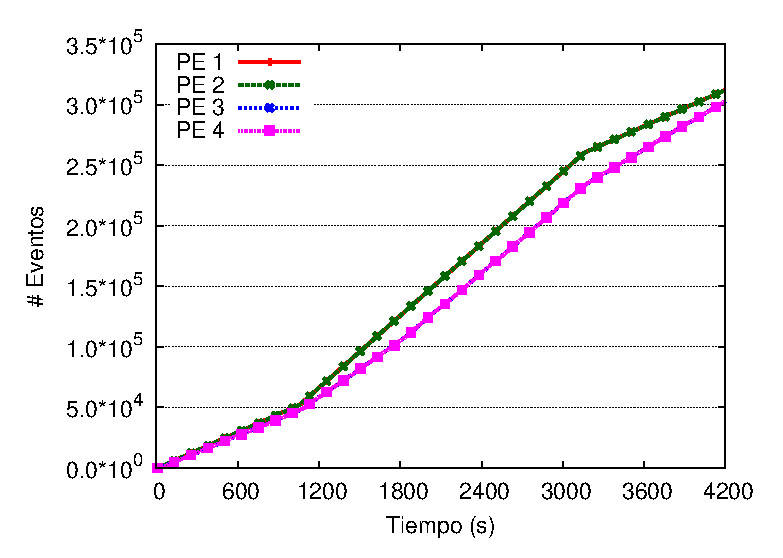
\includegraphics[scale=0.7]{images/exp/app1/normal/cm/eventCount.eps}
    \caption{Cantidad total de eventos procesados en la primera aplicación con un envío variable de la fuente de datos con uso del modelo.}
    \label{fig:app1-normal-eventCount-cm}
\end{figure}

\begin{figure}[!ht]
\centering
    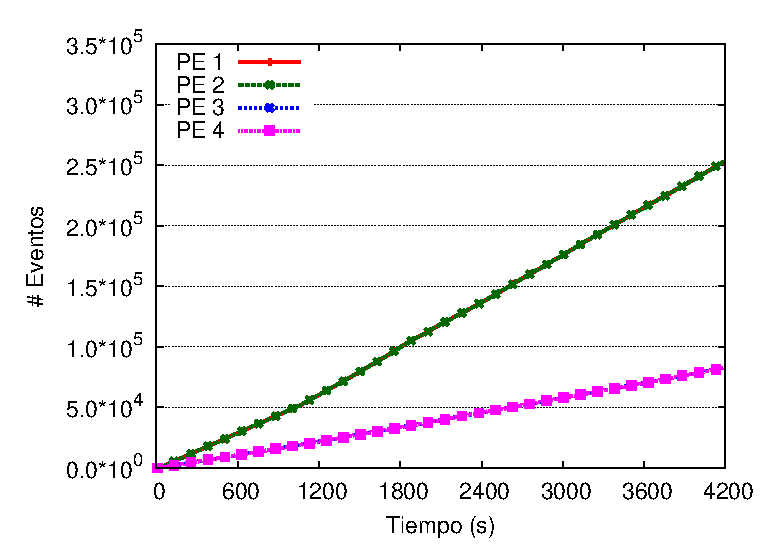
\includegraphics[scale=0.7]{images/exp/app1/normal/sm/eventCount.eps}
    \caption{Cantidad total de eventos procesados en la primera aplicación con un envío variable de la fuente de datos sin uso del modelo.}
    \label{fig:app1-normal-eventCount-sm}
\end{figure}

\subsection{Aplicación 2: Contador de palabras en muestras de textos}
En la segunda aplicación se ha procedido a realizar dos experimentos, los cuales son similares a los anteriores. En el primer experimento se realiza un envío constante de los eventos, y en el segundo, un envío variable. En ambos experimentos, se han realizado dos pruebas, donde la primera consiste en la ejecución de la aplicación en un sistema SPS que usa el modelo elástico, y la segunda sin el uso de éste.

\normalsize{Para el análisis de los experimentos, se ha considerado el rendimiento y la cantidad de réplicas del grafo y la cantidad total de eventos procesados. En el Anexo} \ref{apendice:estadisticas-operadores} \normalsize{se presentan las estadísticas de cada uno de los operadores.}

%%% EXP2 CONSTANTE - OPERADORES %%%

%En las Figuras \ref{fig:app2-uniform-statusSplitPE-cm} y \ref{fig:app2-uniform-statusSplitPE-sm} se observan las estadísticas del PE Split con y sin uso del modelo respectivamente con un flujo constante de eventos. En el primer gráfico la tasa de llegada de los primeros 200 segundos se encuentran ciertos \textit{peak}, los cuales se deben al retraso en la toma de estadísticas, producto de la replicación del PE Counter como se aprecia en la Figura \ref{fig:app2-uniform-statusCounterPE-cm}. Independiente del uso del modelo, se observa que el comportamiento entre los dos PEs es prácticamente igual, y eso se debe a la baja carga que posee el PE. Esto se debe a que este operador es auxiliar, por lo que el costo de separar las palabras y enviarlo a las distintas réplicas del siguiente operador, el cual posee estado, es de bajo costo computacional.
%
%En cambio, en las Figuras \ref{fig:app2-uniform-statusCounterPE-cm} y \ref{fig:app2-uniform-statusCounterPE-sm} se observa una diferencia en los rendimientos del PE Counter. Esto se debe a que este operador posee un alto costo computacional, debido al gran tamaño de la bolsa de palabras que se usa para comparar con las palabras del \textit{tweets}. Debido a esto, al generar las réplicas, se produce una mejora considerable del operador en los primeros 100 segundo.
%
%En este caso, el predictor se activa dado que se realiza un aumento de 9 a 14 réplicas. Si bien, la cantidad de réplicas fue alta, no se considera el operador en estado ocioso, dado que el promedio de tasa de procesamiento posterior al segundo 100 es de 0.63, por lo que no se disminuye la cantidad de réplicas.
%
%Dentro de las observaciones importantes a destacar, se encuentra el procesamiento del PE Counter, el cual al procesar los eventos, deja algunos en cola para posteriormente ser procesados, independiente si se añaden más réplicas, lo cual se puede observar en la cola que se muestra en la Figura \ref{fig:app2-uniform-statusCounterPE-cm}. Si bien, se generan colas con el uso del modelo, es menos de la mitad de las colas que surgen sin el uso del modelo. Este problema surge debido a la implementación en el SPS S4, debido que los PEs no procesan la cantidad de eventos que deben procesar en un período de tiempo. Esto no significa que se pierden eventos, sino que en caso de no procesarlos los deja en cola para posteriormente procesarlos. Por lo que si no se envían más eventos de la fuente de datos, los eventos en cola se procesan hasta vaciar el \textit{buffer}.
%
%En el último PE, se observa que existe una baja cantidad de eventos entrantes, como se muestra en las Figuras \ref{fig:app2-uniform-statusMergePE-cm} y \ref{fig:app2-uniform-statusMergePE-sm}, debido a su condición de operador auxiliar. Cabe recordar que se denomina operador auxiliar a los PEs predecesor y sucesores del posible operador sobrecargado, de esta manera, estos operadores se dedican a dividir la información para enviarla a las distintas réplicas del operador, y posteriormente juntar la información obtenida por las distintas réplicas de éste. La baja cantidad de eventos entrantes se debe a que los eventos entrantes sólo son enviados cada 10 segundos por el PE Counter. En el primer gráfico, se observa que la tasa de llegada aumenta posterior a los 100 segundos, debido a la replicación del operador predecesor. En cambio, en el segundo gráfico, el flujo de entrada sólo se condiciona por una réplica, por lo que no existe un aumento de la tasa de llegada. Cabe destacar que el sistema con modelo si genera colas, a diferencia del sin modelo, y esto se debe a que al procesar mayor cantidad de eventos, surge el problema de procesamiento descrito anteriormente, debido a la implementación realizada en el SPS S4.

%\begin{figure}[p]
%\centering
%    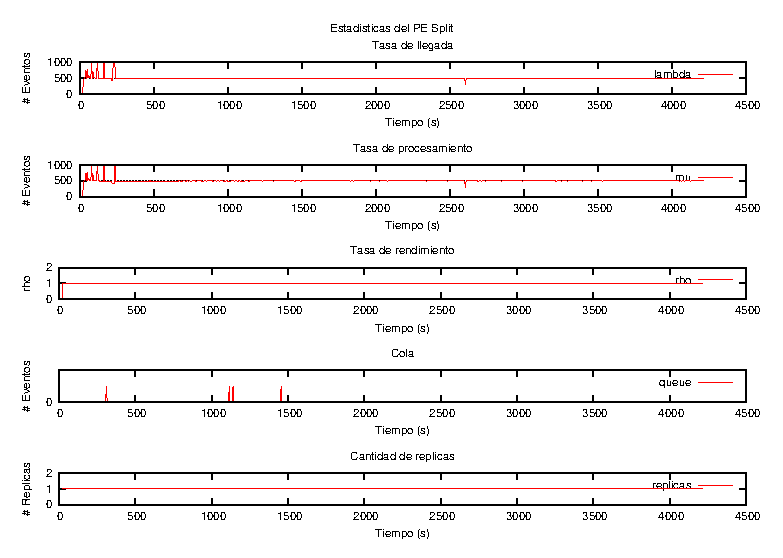
\includegraphics[scale=1.1]{images/exp/app2/uniform/cm/statusSplitPE.eps}
%    \caption{Estadísticas del PE Split en la segunda aplicación con un envío constante de la fuente de datos con uso del modelo.}
%    \label{fig:app2-uniform-statusSplitPE-cm}
%\end{figure}
%
%\begin{figure}[p]
%\centering
%    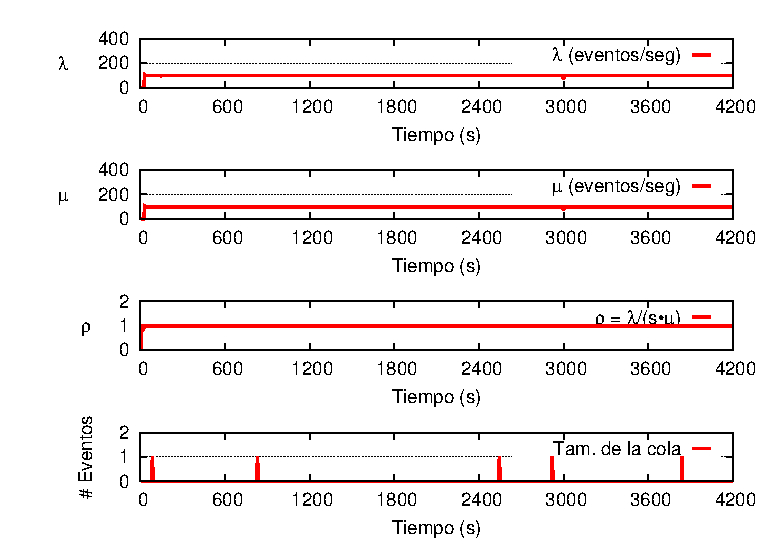
\includegraphics[scale=1.1]{images/exp/app2/uniform/sm/statusSplitPE.eps}
%    \caption{Estadísticas del PE Split en la segunda aplicación con un envío constante de la fuente de datos sin uso del modelo.}
%    \label{fig:app2-uniform-statusSplitPE-sm}
%\end{figure}
%
%\begin{figure}[p]
%\centering
%    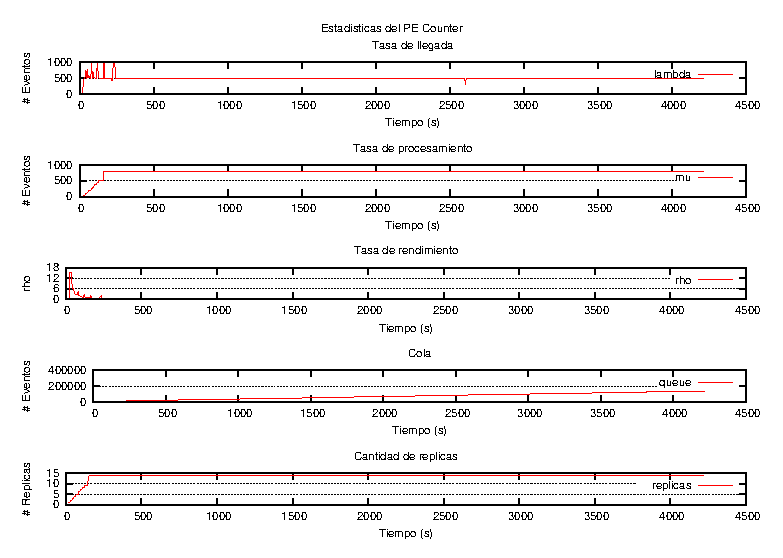
\includegraphics[scale=1.1]{images/exp/app2/uniform/cm/statusCounterPE.eps}
%    \caption{Estadísticas del PE Counter en la segunda aplicación con un envío constante de la fuente de datos con uso del modelo.}
%    \label{fig:app2-uniform-statusCounterPE-cm}
%\end{figure}
%
%\begin{figure}[p]
%\centering
%    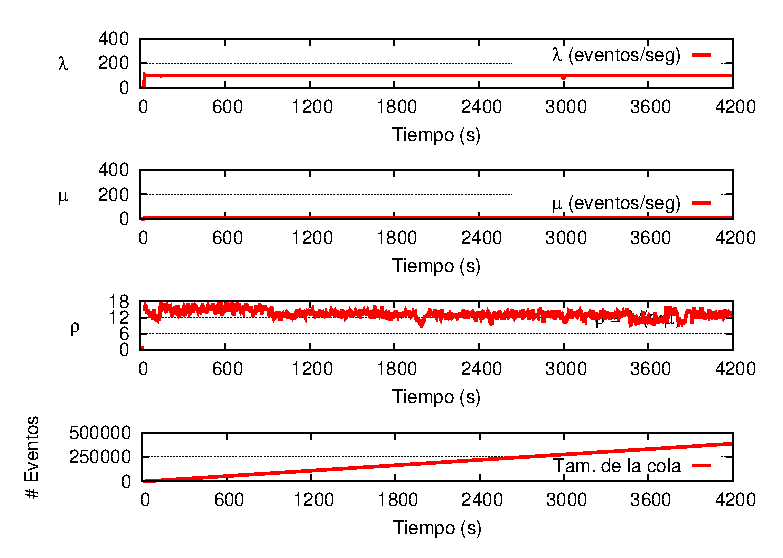
\includegraphics[scale=1.1]{images/exp/app2/uniform/sm/statusCounterPE.eps}
%    \caption{Estadísticas del PE Counter en la segunda aplicación con un envío constante de la fuente de datos sin uso del modelo.}
%    \label{fig:app2-uniform-statusCounterPE-sm}
%\end{figure}
%
%\begin{figure}[p]
%\centering
%    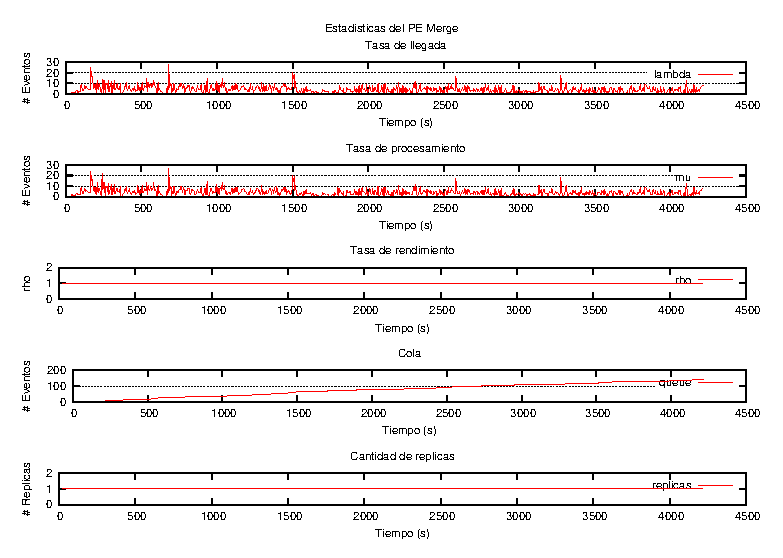
\includegraphics[scale=1.1]{images/exp/app2/uniform/cm/statusMergePE.eps}
%    \caption{Estadísticas del PE Merge en la segunda aplicación con un envío constante de la fuente de datos con uso del modelo.}
%    \label{fig:app2-uniform-statusMergePE-cm}
%\end{figure}
%
%\begin{figure}[p]
%\centering
%    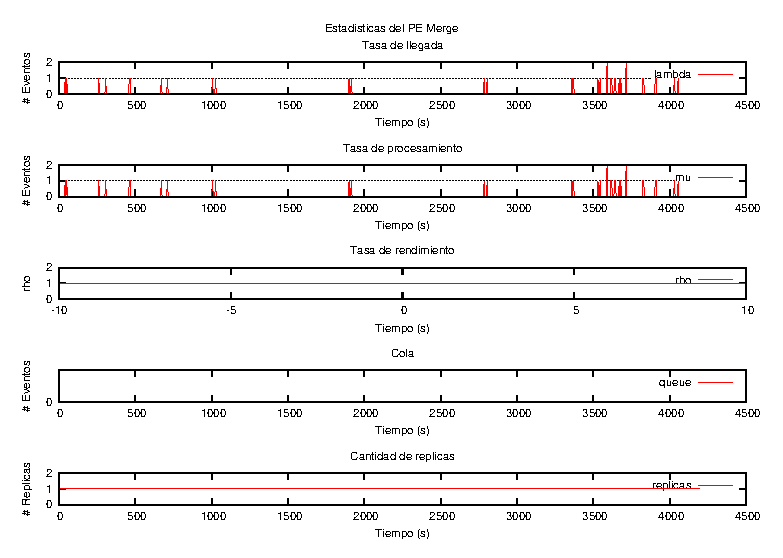
\includegraphics[scale=1.1]{images/exp/app2/uniform/sm/statusMergePE.eps}
%    \caption{Estadísticas del PE Merge en la segunda aplicación con un envío constante de la fuente de datos sin uso del modelo.}
%    \label{fig:app2-uniform-statusMergePE-sm}
%\end{figure}

%%% EXP2 CONSTANTE - PERFORMANCE %%%

La Figura \ref{fig:app2-uniform-processSystem-cm} \normalsize{corresponde al primer experimento y muestra el flujo de datos entrantes del sistema, y como varía la cantidad de réplicas totales del grafo según el flujo de datos.} En esta figura \normalsize{se observa que al principio de la ejecución de la aplicación, existen altas variaciones con el flujo de eventos entrante, y eso se debe a que al crear una réplica del operador sobrecargado, el PE Counter} (véase Anexo \ref{apendice:estadisticas-operadores}), \normalsize{genera una sobrecarga a nivel físico en la máquina, habiendo retrasos en el procesamiento de los datos, lo cual no afecta en el análisis del grafo lógico. Por otra parte, en este experimento se muestra una replicación basado en el algoritmo predictivo, lo cual se debe al análisis del rendimiento del operador según la tasa de rendimiento del PE Counter.}

\begin{figure}[!ht]
	\centering
	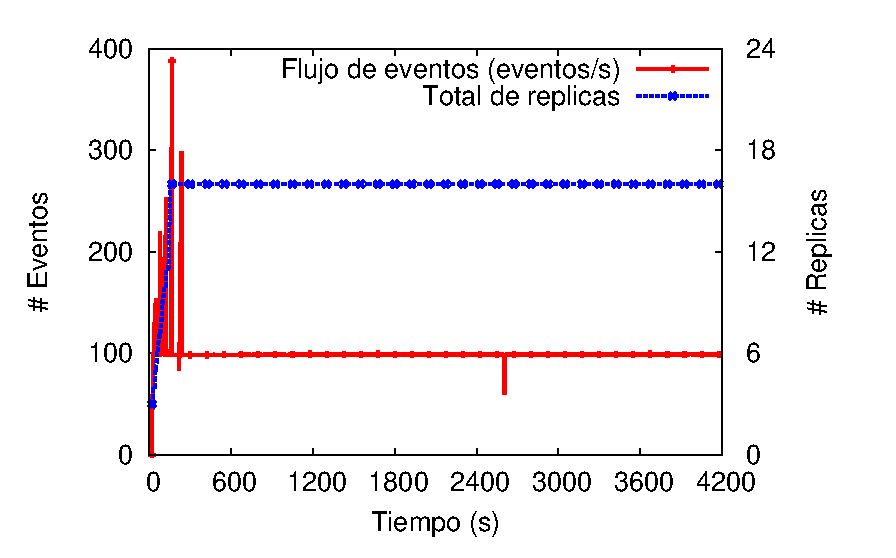
\includegraphics[scale=0.7]{images/exp/app2/uniform/cm/processSystem.eps}
    \caption{Flujo de datos y cantidad de réplicas totales del grafo en la primera aplicación con envío variable de la fuente de datos con uso del modelo.}
	\label{fig:app2-uniform-processSystem-cm}
\end{figure}

%\begin{figure}[!ht]
%	\centering
%	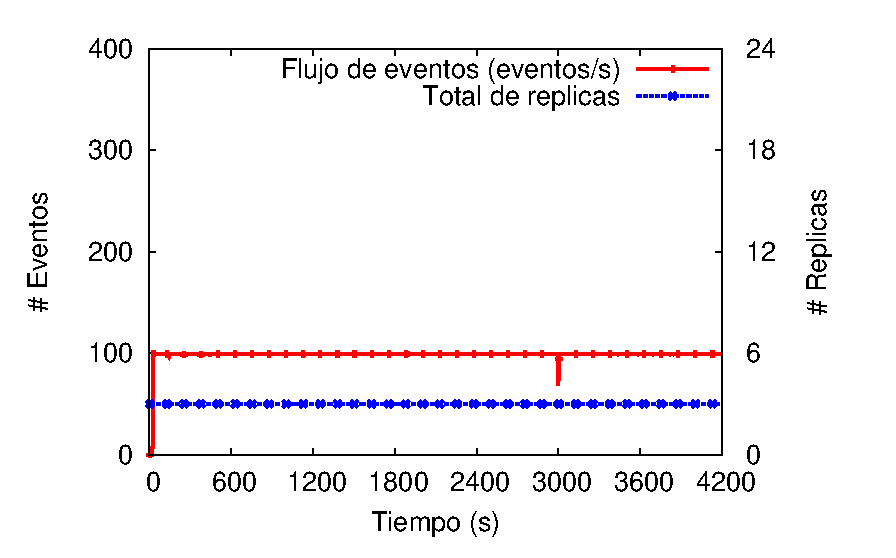
\includegraphics[scale=0.7]{images/exp/app2/uniform/sm/processSystem.eps}
%    \caption{Rendimiento y cantidad de réplicas totales del grafo en la primera aplicación con envío variable de la fuente de datos sin uso del modelo.}
%	\label{fig:app2-uniform-processSystem-sm}
%\end{figure}

%%% EXP2 CONSTANTE - EVENTOS TOTALES %%%

Por otra parte, en las Figuras \ref{fig:app2-uniform-eventCount-cm} y \ref{fig:app2-uniform-eventCount-sm} se muestra la cantidad total de eventos procesados. En el primer gráfico se observa que la diferencia de la pendiente entre las rectas del primer y segundo PE, es menor que en el segundo gráfico. Esto se debe al aumento de la cantidad de réplicas, por lo que se puede procesar mayor cantidad de eventos, alcanzando un total de 275.290 eventos con uso el modelo contra 28.152 sin uso del modelo. En este caso se logro procesar hasta 9 veces mas eventos haciendo uso del modelo elástico.

Dentro de las observaciones importantes está lo ocurrido en la Figura \ref{fig:app2-uniform-eventCount-cm}, donde no existe una mejora por parte del segundo PE de manera paralela al flujo de datos emanado por el primer PE. Como se había explicado anteriormente, independiente que se generen más réplicas, los operadores igualmente van a encolar debido a la sobrecarga surgida por parte de la máquina física.

En el PE 3 (PE Merge) se presenta una baja cantidad de eventos procesados, lo cual se observa en las Figuras \ref{fig:app2-uniform-eventCount-cm} y \ref{fig:app2-uniform-eventCount-sm}. Esto se debe a su condición de operador auxiliar. Cabe recordar que se denomina operador auxiliar a los PEs predecesor y sucesores de un operador con estado, de esta manera, estos operadores se dedican a dividir la información para enviarla a las distintas réplicas del operador, y posteriormente juntar la información obtenida por las distintas réplicas de éste. La baja cantidad de eventos entrantes se debe a que los eventos entrantes sólo son enviados cada 10 segundos por el PE 2 (PE Counter), y en caso de procesar mayor cantidad de datos y poseer mayor cantidad de réplicas de este operador, mayor es la cantidad de eventos procesados por el PE 3. Por último, en la aplicación con uso del modelo elástico se han procesado 3.491 eventos, contra 34 eventos procesados sin el modelo elástico.

\begin{figure}[!ht]
\centering
    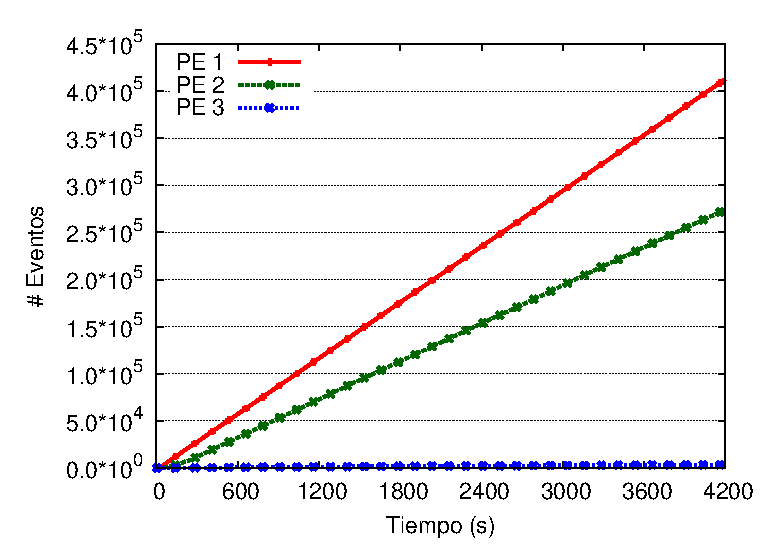
\includegraphics[scale=0.7]{images/exp/app2/uniform/cm/eventCount.eps}
    \caption{Cantidad total de eventos procesados en la segunda aplicación con un envío constante de la fuente de datos sin uso del modelo.}
    \label{fig:app2-uniform-eventCount-cm}
\end{figure}

\begin{figure}[!ht]
\centering
    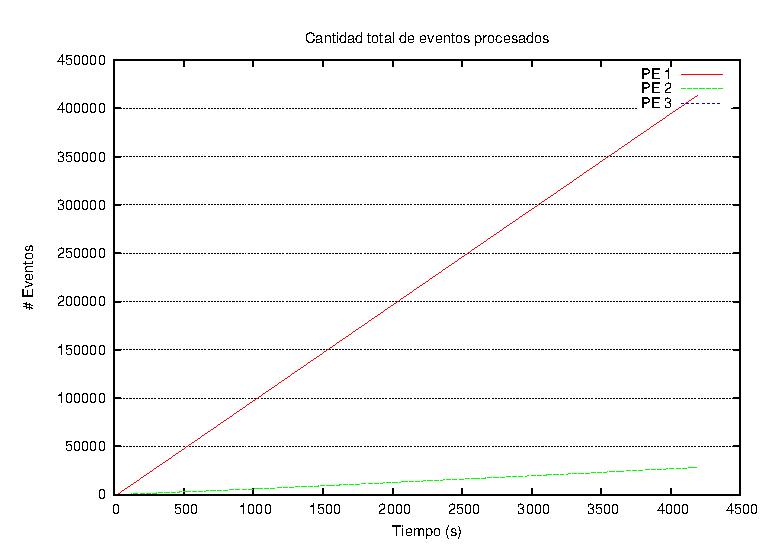
\includegraphics[scale=0.7]{images/exp/app2/uniform/sm/eventCount.eps}
    \caption{Cantidad total de eventos procesados en la segunda aplicación con un envío constante de la fuente de datos con uso del modelo.}
    \label{fig:app2-uniform-eventCount-sm}
\end{figure}

%%% EXP2-VARIACIONES OPERADORES %%%

%En las Figuras \ref{fig:app2-uniform-statusSplitPE-cm} y \ref{fig:app2-uniform-statusSplitPE-sm} se observan las estadísticas del PE Split con y sin uso del modelo respectivamente con un flujo variable de eventos. Como se mencionó anteriormente, en las estadísticas recuperadas de la aplicación haciendo uso del modelo se pueden observar \textit{peaks}, los cuales son provocados por la replicación del siguiente operador. Sin embargo, estos \textit{peaks} no impactan el rendimiento del sistema haciendo uso del modelo propuesto. Debido que el PE Split posee un bajo nivel de cómputo, no existe una tasa de rendimiento que sea inestable, tanto para el sistema con y sin uso del modelo, por lo que no se presentan sobrecargas.
%
%A diferencia del PE Split, en el PE Counter si existe un nivel de sobrecarga, como se observar en las Figuras \ref{fig:app2-normal-statusCounterPE-cm} y \ref{fig:app2-normal-statusCounterPE-sm}. En el primer gráfico se aprecia que en los primeros 100 segundos existe una inestabilidad en el sistema, sin embargo, posteriormente se alcanza estabilidad utilizando el modelo, dado que se replica el operador. Esta inestabilidad se vuelve a apreciar en el segundo 1100, cuando aumenta el envío de eventos desde la fuente de datos, lo cual hace que la cantidad de réplicas existentes sean insuficientes, volviendo a replicar el operador. Y finalmente, en el último tramo disminuye la cantidad de réplicas en el segundo 3200, debido que el envío de datos disminuye.
%
%Como se explicó en el experimento de envío variable de la fuente de datos en la aplicación 1, la cantidad óptima de operadores en el primer tramo es distinta a la del tercer tramo. Esto se debe a que en el primer tramo aumenta la cantidad de réplicas para ir convergiendo $\rho$ a un valor de 1, en cambio, en el tercer tramo disminuye la cantidad de réplicas para ir convergiendo $\rho$ a 0.5, límite inferior para definir el estado estable.
%
%Por otra parte, en este experimento no se ha activado el predictor, y esto se debe a que la replicación fue paulatina. Por lo tanto, el operador alcanza una convergencia de la cantidad de réplicas necesarias, por lo que al predecir se determina que el operador se encuentra estable a futuro.
%
%En el tercer PE, se analiza que la tasa de llegada es baja tanto en las Figuras \ref{fig:app2-normal-statusMergePE-cm} y \ref{fig:app2-normal-statusMergePE-sm}, y esto se debe a que este PE es auxiliar como se explicó en el anterior experimento, por lo que le llegan eventos cada 10 segundos por cada réplica del PE Counter. El análisis que se realiza en el PE Merge es el mismo explicado en el anterior experimento, donde la tasa de llegada va a depender de la cantidad de réplicas existentes en el PE Counter, por lo que la tasa de llegada es mayor en el sistema con modelo.

%\begin{figure}[p]
%\centering
%    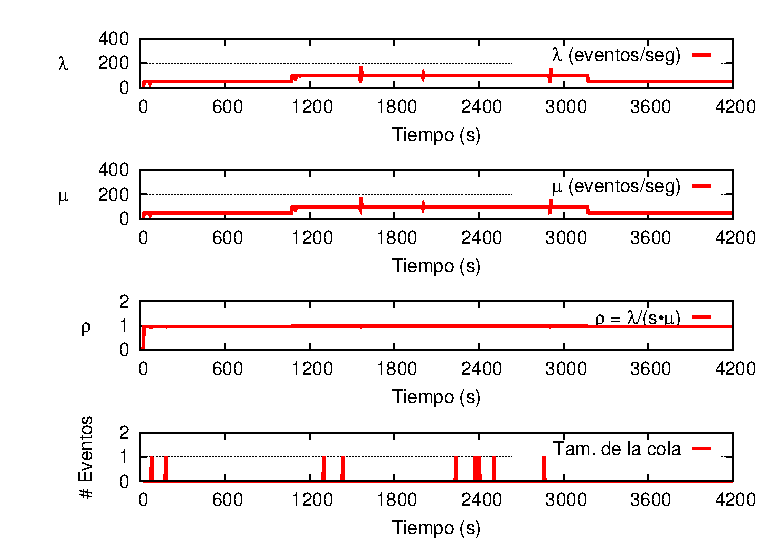
\includegraphics[scale=1.1]{images/exp/app2/normal/cm/statusSplitPE.eps}
%    \caption{Estadísticas del PE Split en la segunda aplicación con un envío variable de la fuente de datos con uso del modelo.}
%    \label{fig:app2-normal-statusSplitPE-cm}
%\end{figure}
%
%\begin{figure}[p]
%\centering
%    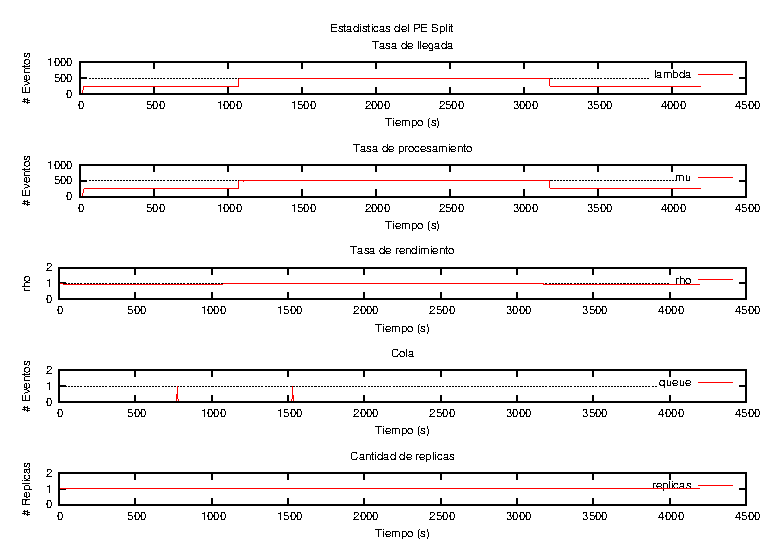
\includegraphics[scale=1.1]{images/exp/app2/normal/sm/statusSplitPE.eps}
%    \caption{Estadísticas del PE Split en la segunda aplicación con un envío variable de la fuente de datos sin uso del modelo.}
%    \label{fig:app2-normal-statusSplitPE-sm}
%\end{figure}
%
%\begin{figure}[p]
%\centering
%    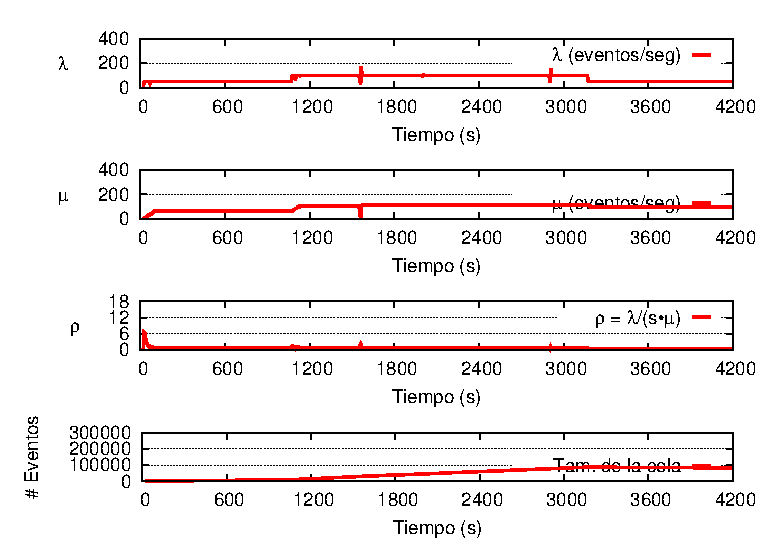
\includegraphics[scale=1.1]{images/exp/app2/normal/cm/statusCounterPE.eps}
%    \caption{Estadísticas del PE Counter en la segunda aplicación con un envío variable de la fuente de datos con uso del modelo.}
%    \label{fig:app2-normal-statusCounterPE-cm}
%\end{figure}
%
%\begin{figure}[p]
%\centering
%    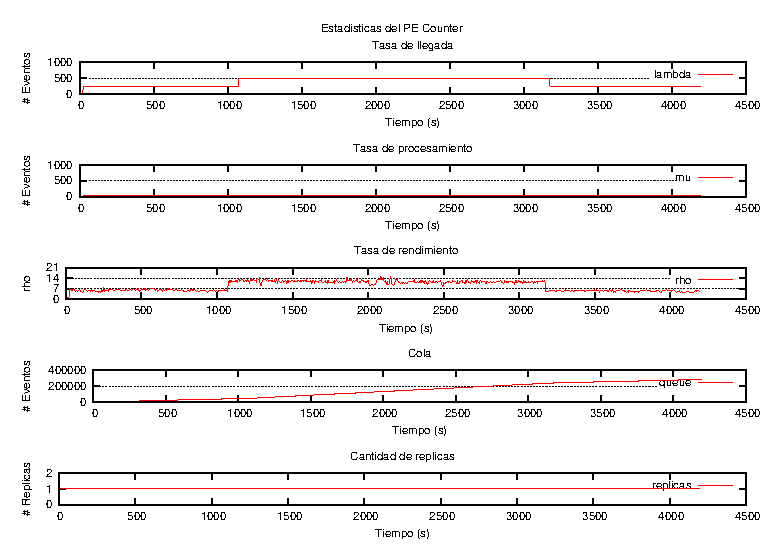
\includegraphics[scale=1.1]{images/exp/app2/normal/sm/statusCounterPE.eps}
%    \caption{Estadísticas del PE Counter en la segunda aplicación con un envío variable de la fuente de datos sin uso del modelo.}
%    \label{fig:app2-normal-statusCounterPE-sm}
%\end{figure}
%
%\begin{figure}[p]
%\centering
%    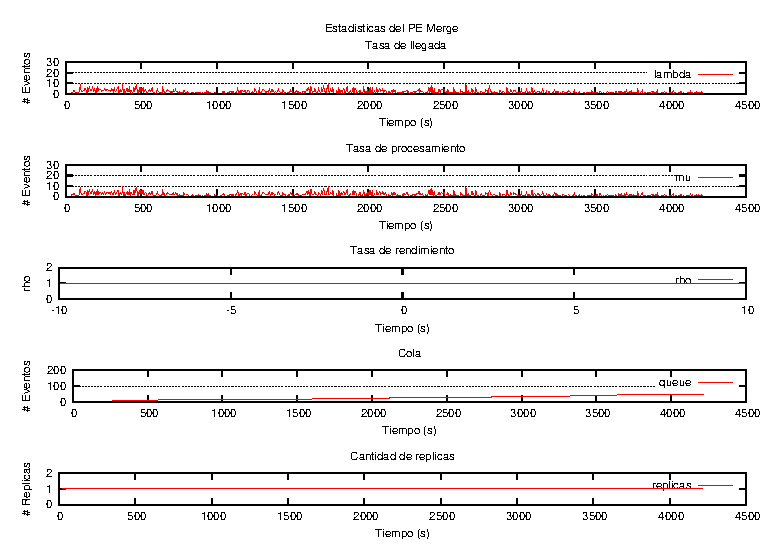
\includegraphics[scale=1.1]{images/exp/app2/normal/cm/statusMergePE.eps}
%    \caption{Estadísticas del PE Merge en la segunda aplicación con un envío variable de la fuente de datos con uso del modelo.}
%    \label{fig:app2-normal-statusMergePE-cm}
%\end{figure}
%
%\begin{figure}[p]
%\centering
%    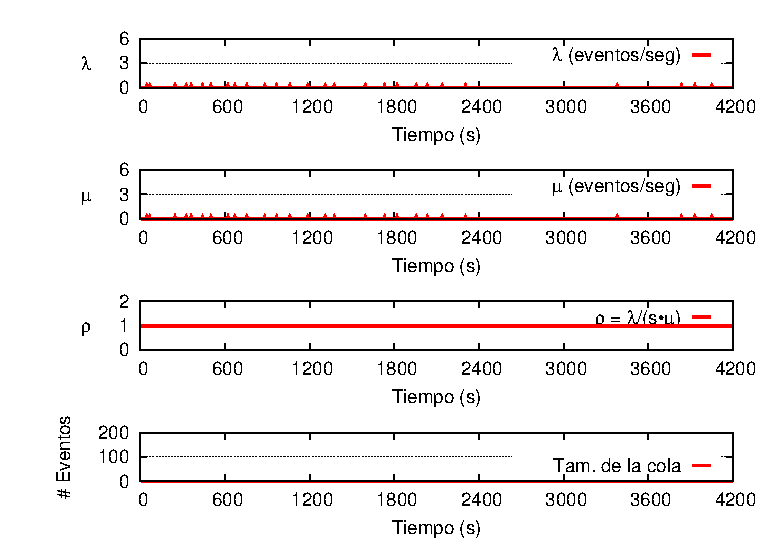
\includegraphics[scale=1.1]{images/exp/app2/normal/sm/statusMergePE.eps}
%    \caption{Estadísticas del PE Merge en la segunda aplicación con un envío variable de la fuente de datos sin uso del modelo.}
%    \label{fig:app2-normal-statusMergePE-sm}
%\end{figure}

%%% EXP2-VARIABLE PERFORMANCE %%%

La Figura \ref{fig:app2-normal-processSystem-cm} \normalsize{corresponde al primer experimento y muestra el flujo de datos entrantes del sistema, y como varía la cantidad de réplicas totales del grafo según el flujo de datos.} En esta figura \normalsize{se puede observar como el número de réplicas se adapta al tráfico recibido. En el primer y segundo tercio se muestra un aumento de réplicas, pero posteriormente en el último disminuye, aprovechando los recursos que se disponen. A diferencia del experimento anterior, en éste no se activa el algoritmo predictivo, y eso se debe a qué no existe una posible sobrecarga a futuro, dado que se estabiliza el sistema antes de este análisis debido al algoritmo reactivo.}

\begin{figure}[!ht]
	\centering
	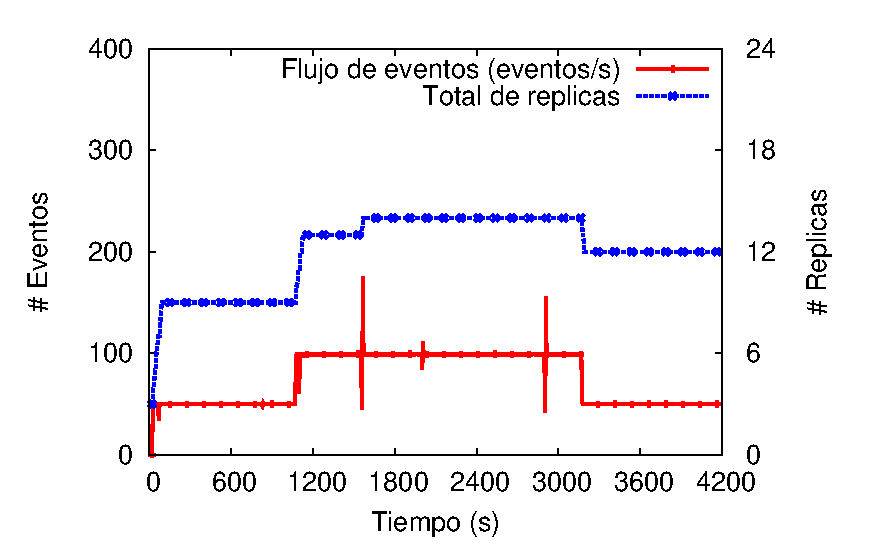
\includegraphics[scale=0.7]{images/exp/app2/normal/cm/processSystem.eps}
    \caption{Flujo de datos y cantidad de réplicas totales del grafo en la primera aplicación con envío variable de la fuente de datos con uso del modelo.}
	\label{fig:app2-normal-processSystem-cm}
\end{figure}

%%% EXP2-VARIABLE EVENTOS TOTALES %%%

Por otro lado, en las Figuras \ref{fig:app2-normal-eventCount-cm} y \ref{fig:app2-normal-eventCount-sm} se muestra la cantidad total de eventos procesados. En el primer gráfico se aprecia que la curva del primer PE y el segundo PE es más cercana que las del segundo gráfico, y esto se debe a la replicación que se ha efectuado en el sistema. Cabe destacar que el sistema con uso del modelo ha procesado un total de 228.942 eventos, mientras que el sistema sin uso del modelo ha procesado 27.751 eventos. Por lo que la solución permite aumentar en más de 8 veces la cantidad de eventos procesados.

El análisis que se realiza en el PE 3 (PE Merge) es el mismo explicado en el anterior experimento, donde la cantidad de eventos procesados va a depender de la cantidad de réplicas existentes en el PE 2 (PE Counter). Por último, se ha realizado un procesamiento de 1.578 eventos con uso del modelo, y 27 eventos sin uso del modelo.

\begin{figure}[!ht]
	\centering
    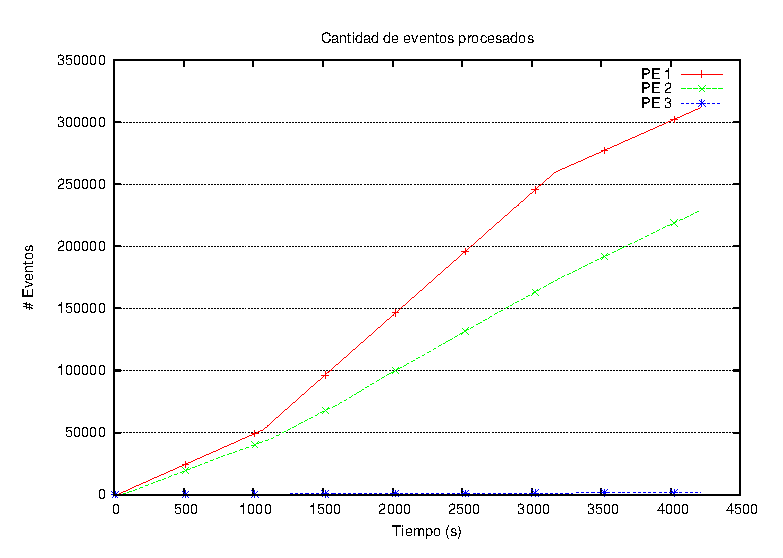
\includegraphics[scale=0.7]{images/exp/app2/normal/cm/eventCount.eps}
    \caption{Cantidad total de eventos procesados en la segunda aplicación con un envío variable de la fuente de datos con uso del modelo.}
    \label{fig:app2-normal-eventCount-cm}
\end{figure}

\begin{figure}[!ht]
	\centering
    \includegraphics[scale=0.7]{images/exp/app2/normal/sm/eventCount.eps}
    \caption{Cantidad total de eventos procesados en la segunda aplicación con un envío variable de la fuente de datos sin uso del modelo.}
    \label{fig:app2-normal-eventCount-sm}
\end{figure}

\subsection{Aplicación 3: Aplicación sintética}
En la tercera aplicación se ha procedido a realizar un experimento que consta de dos pruebas, al igual que en las anteriores pruebas, donde una de ellas hace uso del modelo elástico y la otra no. Ambas pruebas se han realizado con un envío constante de 100 eventos por segundo desde la fuente de datos.

Para el análisis de los experimentos, se ha considerado el consumo de memoria, el uso de la CPU, \normalsize{el rendimiento, la cantidad de réplicas del grafo} y la cantidad total de eventos procesados. En el Anexo \ref{apendice:estadisticas-operadores} \normalsize{se presentan las estadísticas de cada uno de los operadores.}

%%% EXP3 - CPU %%%

Respecto a la utilización de CPU, se puede observar en las Figuras \ref{fig:app3-consumeCPU-cm} y \ref{fig:app3-consumeCPU-sm} el porcentaje de uso con y sin uso del modelo respectivamente. Si bien la diferencia no es significante en el uso de la CPU por parte de la aplicación, en el primer caso existe un promedio de $0.62\%$ de utilización de CPU, contra un promedio de $0.61\%$ de uso en el segundo caso, habiendo un aumento del $0,01\%$ de utilización promedio de CPU. Dentro de los primeros 10 segundo existe un alto uso de CPU en ambos gráficos, lo que se debe al despliegue y compilación de la aplicación en el sistema de S4.

\begin{figure}[!ht]
\centering
    \includegraphics[scale=0.75]{images/exp/app3/cm/fisical/consumeCPU.eps}
    \caption{Porcentaje de utilización de la CPU en la tercera aplicación con uso del modelo.}
    \label{fig:app3-consumeCPU-cm}
\end{figure}

\begin{figure}[!ht]
\centering
    \includegraphics[scale=0.75]{images/exp/app3/sm/fisical/consumeCPU.eps}
    \caption{Porcentaje de utilización de la CPU en la tercera aplicación sin uso del modelo.}
    \label{fig:app3-consumeCPU-sm}
\end{figure}

%%% EXP3 - RAM %%%

Por otra parte, el consumo de memoria RAM es presentado por las Figuras \ref{fig:app3-consumeRAM-cm} y \ref{fig:app3-consumeRAM-sm}, donde la primera es con uso de modelo y la segunda sin uso. En el primer gráfico existe un consumo promedio de $264$ MB versus $268$ MB del segundo gráfico, habiendo una disminución del $1,5\%$ de consumo de memoria RAM. En el primer gráfico se observa un aumento del consumo de memoria en el segundo 200, a diferencia del segundo gráfico, debido al mayor consumo de eventos y creación de nuevos operadores. Posterior al segundo 600, por parte del sistema sin uso del modelo, se muestra un aumento del consumo de memoria, lo cual se debe a la cantidad de eventos en la cola que existen en el sistema, a diferencia del primer gráfico que hubo una convergencia en el consumo de la memoria, por lo que posteriormente al reducir las colas, reduce igualmente el consumo de memoria principal en la ejecución.

\begin{figure}[!ht]
\centering
    \includegraphics[scale=0.75]{images/exp/app3/cm/fisical/consumeRAM.eps}
    \caption{Consumo de memoria RAM en la tercera aplicación con uso del modelo.}
    \label{fig:app3-consumeRAM-cm}
\end{figure}

\begin{figure}[!ht]
\centering
    \includegraphics[scale=0.75]{images/exp/app3/sm/fisical/consumeRAM.eps}
    \caption{Consumo de memoria RAM en la tercera aplicación sin uso del modelo.}
    \label{fig:app3-consumeRAM-sm}
\end{figure}

%%% EXP3 - PERFORMANCE

En las Figuras \ref{fig:app3-processSystem-cm} y \ref{fig:app3-processSystem-sm} \normalsize{corresponden al rendimiento que posee el sistema, y como éste varía la cantidad de réplicas totales del grafo según la tasa de entrada.} En la Figura \ref{fig:app3-processSystem-cm} \normalsize{se observa que existe un incremento en la cantidad de réplicas, debido a la sobrecarga de los operadores del grafo} (véase Anexo \ref{apendice:estadisticas-operadores}), \normalsize{aumentando el rendimiento de éste, de tal manera de procesar 97 eventos por segundo en promedio con el uso del modelo. En cambio, en la Figura} \ref{fig:app3-processSystem-sm} \normalsize{no existe un aumento en el rendimiento, teniendo una tasa de salida promedio de 33 eventos por segundo. De esta manera, existe una mejora de 2 veces más eventos procesados con el uso del modelo propuesto.}

\begin{figure}[!ht]
	\centering
	\includegraphics[scale=0.7]{images/exp/app3/cm/logical/processSystem.eps}
    \caption{Rendimiento y cantidad de réplicas totales del grafo en la tercera aplicación con uso del modelo.}
	\label{fig:app3-processSystem-cm}
\end{figure}

\begin{figure}[!ht]
	\centering
	\includegraphics[scale=0.7]{images/exp/app3/sm/logical/processSystem.eps}
    \caption{Rendimiento y cantidad de réplicas totales del grafo en la tercera aplicación sin uso del modelo.}
	\label{fig:app3-processSystem-sm}
\end{figure}

En cuanto a la cantidad total de eventos procesados, en las Figuras \ref{fig:app3-eventCount-cm} y \ref{fig:app3-eventCount-sm} se aprecia que la cantidad de eventos procesados es mayor en el primero gráfico, el cual hace uso del modelo elástico. En el primer gráfico existe un total de 88.169 eventos procesados y en el segundo un total de 29.714 eventos procesados, existiendo una mejora de 3 veces la cantidad de eventos procesados.

\begin{figure}[!ht]
\centering
    \includegraphics[scale=0.75]{images/exp/app3/cm/logical/eventCount.eps}
    \caption{Cantidad de eventos procesados en la tercera aplicación con uso del modelo.}
    \label{fig:app3-eventCount-cm}
\end{figure}

%%% EXP 3 - TIEMPO ALGORITMOS %%%

Finalmente, en la Tabla \ref{tab:tiempo-algoritmos} se muestra el tiempo promedio de ejecución de cada uno de los algoritmos para el análisis de un operador. Se puede observar que si bien el algoritmo predictivo posee un tiempo de ejecución mayor que el algoritmo reactivo, no produce una sobrecarga en el modelo elástico.

\begin{table}[!ht]
\centering
\begin{tabular}{| c | c |}
\hline
Algoritmo & Tiempo (ms) \\ \hline
Reactivo & 0.03 \\
Predictivo & 4.63 \\ \hline
\end{tabular}
\caption{Tiempos de ejecución de los algoritmos del modelo elástico.}
\label{tab:tiempo-algoritmos}
\end{table}

\clearpage
\begin{figure}[!ht]
\centering
    \includegraphics[scale=0.75]{images/exp/app3/sm/logical/eventCount.eps}
    \caption{Cantidad de eventos procesados en la tercera aplicación sin uso del modelo.}
    \label{fig:app3-eventCount-sm}
\end{figure}

%%% EXP3 - OPERADORES %%%

%Finalmente, en las Figuras \ref{fig:app3-statusOnePE-cm} y \ref{fig:app3-statusOnePE-sm} se presentan las estadísticas del primer PE con y sin uso del modelo respectivamente, en los cuales se muestra una diferencia en la tasa de procesamiento en las pruebas con y sin uso del modelo, que afecta en la tasa de llegada del segundo PE como se muestra en las Figura \ref{fig:app3-statusTwoPE-cm} y \ref{fig:app3-statusTwoPE-sm}. Finalmente, en las Figuras \ref{fig:app3-statusThreePE-cm} y \ref{fig:app3-statusThreePE-sm} se presenta el tercer PE, en el cual no existe variación en su tasa de rendimiento en ninguno de los dos casos, debido que en el experimento sin uso del modelo recibe una menor tasa de llegada, dada la tasa de procesamiento del PE anterior.
%
%\begin{figure}[!htp]
%\centering
%    \includegraphics[scale=1]{images/exp/app3/cm/logical/statusOnePE.eps}
%    \caption{Estadísticas del primer PE en la tercera aplicación con un envío constante de la fuente de datos con uso del modelo.}
%    \label{fig:app3-statusOnePE-cm}
%\end{figure}
%
%\begin{figure}[!htp]
%\centering
%    \includegraphics[scale=1]{images/exp/app3/sm/logical/statusOnePE.eps}
%    \caption{Estadísticas del primer PE en la tercera aplicación con un envío constante de la fuente de datos sin uso del modelo.}
%    \label{fig:app3-statusOnePE-sm}
%\end{figure}
%
%\begin{figure}[!htp]
%\centering
%	\includegraphics[scale=1]{images/exp/app3/cm/logical/statusTwoPE.eps}
%    \caption{Estadísticas del segundo PE en la tercera aplicación con un envío constante de la fuente de datos con uso del modelo.}
%    \label{fig:app3-statusTwoPE-cm}
%\end{figure}
%
%\begin{figure}[!htp]
%\centering
%    \includegraphics[scale=1]{images/exp/app3/sm/logical/statusTwoPE.eps}
%    \caption{Estadísticas del segundo PE en la tercera aplicación con un envío constante de la fuente de datos sin uso del modelo.}
%    \label{fig:app3-statusTwoPE-sm}
%\end{figure}
%
%\begin{figure}[!htp]
%\centering
%    \includegraphics[scale=1]{images/exp/app3/cm/logical/statusThreePE.eps}
%    \caption{Estadísticas del tercer PE en la tercera aplicación con un envío constante de la fuente de datos con uso del modelo.}
%    \label{fig:app3-statusThreePE-cm}
%\end{figure}
%
%\begin{figure}[!htp]
%\centering
%    \includegraphics[scale=1]{images/exp/app3/sm/logical/statusThreePE.eps}
%    \caption{Estadísticas del tercer PE en la tercera aplicación con un envío constante de la fuente de datos sin uso del modelo.}
%    \label{fig:app3-statusThreePE-sm}
%\end{figure}